% Szglab4
% ===========================================================================
%
% 
% Szglab4
% ===========================================================================
%
\documentclass[11pt,oneside]{scrbook}

\usepackage[utf8]{inputenc}
\usepackage[T1]{fontenc}

\usepackage{fancyhdr}

\usepackage[magyar]{babel}

\usepackage{longtable}

\usepackage[usenames]{color}

\usepackage{float}

\usepackage{times}

\usepackage{listings}

\usepackage{includes/szglab4}

%mi headerjeink

\usepackage{multirow}

\usepackage{graphicx}

\usepackage[export]{adjustbox}

%a mi headerjeinknek a vége


\usepackage[%
	pdftitle={Szglab 4},% A PDF dokumentum címe.
	pdfauthor={X.Y.)},% Szerző(k) neve(i)
	pdfsubject={Szglab 4},% A PDF dokumentum témája
	pdfcreator={MiKTeX, LaTeX with hyperref and KOMA-Script}, % A PDF dokumentum készült ...
	pdfkeywords={Szglab4},% Kulcsszavak
	pdfpagemode=UseOutlines,% Tartalomjegyzék megjelenítése megnyitáskor
	pdfdisplaydoctitle=true,% Fájlnév helyett a dokumentum neve jelenjen meg
	pdflang=hu,% A dokumentum nyelve
	unicode
]{hyperref}

\definecolor{LinkColor}{rgb}{0,0,0}
\definecolor{ListingBackground}{rgb}{1,1,1}

\hypersetup{%
	colorlinks=true,% Színes linkek aktiválása a dokumentumban (keretek nélkül)
	linkcolor=LinkColor,%    szín beállítása
	citecolor=LinkColor,%    szín beállítása
	filecolor=LinkColor,%    szín beállítása
	menucolor=LinkColor,%    szín beállítása
	urlcolor=LinkColor,%     URL hivatkozások színe
	bookmarksnumbered=true
}

%
% ===========================================================================
% EOF
%

%
\csapat{Stapelspeicher}{88}
\konzulens{Simon Balázs}
\taga{Gema Barnabás}{IX7MPR}{gema.barnabas@gmail.com}
\tagb{Juszt Ádám}{XYH6FV}{juszta@gmail.com}
\tagc{Kemény Károly}{WKJAGY}{kemeny.karoly@gmail.com}
\tagd{Pilinszki-Nagy Csongor}{CZIYIA}{pnagycsongi@gmail.com}
\tage{Somogyi Gábor}{FJ4IA9}{gabor.somogyi1@gmail.com}
\datum{\today}
%
\begin{document}
%
% Nem aktuális sorokat kommentezni
%
\fedlap{Prototípus koncepciója} 
%\fedlap{3. Analízis modell kidolgozása 1}
%\fedlap{4. Analízis modell kidolgozása 2}
% ...
%
% Tartalomjegyzék és ábrák jegyzéke
%
\clearpage \tableofcontents \pagestyle{fancy}
\clearpage \listoffigures \pagestyle{fancy}
%
% Nem aktuális fejezetek kikommentezve
%
\setcounter{chapter}{1}
% Szglab4
% ===========================================================================
%
\chapter{Követelmény, projekt, funkcionalitás}

\thispagestyle{fancy}

\section{Bevezetés}

\subsection{Cél}

\comment{A dokumentum célja.}

\subsection{Szakterület}

\comment{A kialakítandó szoftver milyen területen használható, milyen célra.}

\subsection{Definíciók, rövidítések}
\comment{A dokumentumban használt definíciók, rövidítések magyarázata.}

\subsection{Hivatkozások}
\comment{A dokumentumban használt anyagok, web-oldalak felsorolása}

\subsection{Összefoglalás}
\comment{A dokumentum további részeinek rövid ismertetése}

\section{Áttekintés}
\subsection{Általános áttekintés}
\comment{A kialakítandó szoftver legmagasabb szintű architekturális képe. A fontosabb alrendszerek felsorolása, a közöttük kialakítandó interfészek lényege, a felhasználói kapcsolatok alapja. Esetleges hálózati és adattárolási elvárások.}

\subsection{Funkciók}
\comment{A feladat kb. 4000 karakteres (kb 1,5 oldal) részletezettségű magyar nyelvű leírása. Nem szerepelhetnek informatikai kifejezések.}

\subsection{Felhasználók}
\comment{A felhasználók jellemzői, tulajdonságai}

\subsection{Korlátozások}
\comment{Az elkészítendő szoftverre vonatkozó – általában nem funkcionális - előírások, korlátozások.}

\subsection{Feltételezések, kapcsolatok}
\comment{A dokumentumban használt anyagok, web-oldalak felsorolása}

\section{Követelmények}
\subsection{Funkcionális követelmények}


\comment{Az alábbi táblázat kitöltésével készítendő. Dolgozzon ki követelmény azonosító rendszert! Az ellenőrzés módja szokásosan bemutatás és/vagy kiértékelés. Prioritás lehet alapvető, fontos, opcionális. Az alapvető követelmények nem teljesítése végzetes. Forrás alatt a követelményt előíró anyagot, szervezetet kell érteni. Esetünkben forrás lehet maga a csapat is, mikor ő talál ki követelményt. Use-case-ek alatt az adott követelményt megvalósító használati esete(ke)t kell megadni.}

% Azonosító, Leírás, Ellenőrzés, Prioritás, Forrás, Use-case, Komment
\begin{longtable}{| l | l | l | l | l | l | l |}
\hline
\textbf{Azonosító}   & \textbf{Leírás} & \textbf{Ellenőrzés} & \textbf{Prioritás} & \textbf{Forrás} & \textbf{Use-case} & \textbf{Komment} \tabularnewline
\hline\hline
... & ... & ... & ... & ... & ... & ... \tabularnewline
\hline
\end{longtable}

\subsection{Erőforrásokkal kapcsolatos követelmények}

\comment{A szoftver fejlesztésével és használatával kapcsolatos számítógépes, hardveres, alapszoftveres és egyéb architekturális és logisztikai követelmények}

% Azonosító, Leírás, Ellenőrzés, Prioritás, Forrás, Komment
\begin{longtable}{| l | l | l | l | l | l |}
\hline
\textbf{Azonosító}   & \textbf{Leírás} & \textbf{Ellenőrzés} & \textbf{Prioritás} & \textbf{Forrás} & \textbf{Komment} \tabularnewline
\hline\hline
... & ... & ... & ... & ... & ... \tabularnewline
\hline
\end{longtable}


\subsection{Átadással kapcsolatos követelmények}
\comment{A szoftver átadásával, telepítésével, üzembe helyezésével kapcsolatos követelmények}

% Azonosító, Leírás, Ellenőrzés, Prioritás, Forrás, Komment
\begin{longtable}{| l | l | l | l | l | l |}
\hline
\textbf{Azonosító}   & \textbf{Leírás} & \textbf{Ellenőrzés} & \textbf{Prioritás} & \textbf{Forrás} & \textbf{Komment} \tabularnewline
\hline\hline
... & ... & ... & ... & ... & ... \tabularnewline
\hline
\end{longtable}

\subsection{Egyéb nem funkcionális követelmények}
\comment{A biztonsággal, hordozhatósággal, megbízhatósággal, tesztelhetőséggel, a felhasználóval kapcsolatos követelmények}

% Azonosító, Leírás, Ellenőrzés, Prioritás, Forrás, Komment
\begin{longtable}{| l | l | l | l | l | l |}
\hline
\textbf{Azonosító}   & \textbf{Leírás} & \textbf{Ellenőrzés} & \textbf{Prioritás} & \textbf{Forrás} & \textbf{Komment} \tabularnewline
\hline\hline
... & ... & ... & ... & ... & ... \tabularnewline
\hline
\end{longtable}


\section{Lényeges use-case-ek}
\comment{A 2.3.1-ben felsorolt követelmények közül az alapvető és fontos követelményekhez tartozó használati esetek megadása az alábbi táblázatos formában.}
\subsection{Use-case leírások}

\comment{Minden use-case-hez külön}

\usecase{...}{...}{...}{...}

\usecase{...}{...}{...}{...}

\section{Szótár}
\comment{A szótár a követelmények alapján készítendő fejezet. Egy szótári bejegyzés definiálásához csak más szótári bejegyzések és köznapi – a feladattól független – fogalmak használhatók fel. A szótár mérete kb. 1-2 oldal legyen.}

\section{Projekt terv}
\comment{Tartalmaznia kell a projekt végrehajtásának lépéseit, a lépések, eredmények határidejét, az egyes feladatok elvégzéséért felelős személyek nevét és beosztását, a szükséges erőforrásokat, stb. Meg kell adni a csoportmunkát támogató eszközöket, a választott technikákat! Definiálni kell, hogy hogyan történik a dokumentumok és a forráskód megosztása!}



% Szglab4
% ===========================================================================
%
\section{Napló}

\begin{naplo}

\bejegyzes
{2015.02.09.~14:00~} % Kezdet
{1 óra} % Időtartam
{Juszt Ádám\newline
Kemény Károly\newline
Pilinszki-Nagy Csongor\newline
Somogyi Gábor} % Résztvevők
{Meeting. Döntés: Technológiai áttekintés, a fejlesztés során használt szoftverek megismerése.} % Leírás

\bejegyzes
{2015.02.16.~16:00~}
{2 óra}
{Gema Barnabás\newline
	Juszt Ádám\newline
	Kemény Károly\newline
	Pilinszki-Nagy Csongor\newline
	Somogyi Gábor} % Résztvevők}
{Tevékenység: Feladatok kiosztása: Somogyi Gábor: 2.1, napló elkészítése, vezetése, fedlap elkészítése; Juszt Ádám: 2.2, architekturális kép; Pilinszki-Nagy Csongor: 2.3; Gema Barnabás: 2.4; Kemény Károly: 2.5}

\bejegyzes
{2015.02.17.~18.00}
{3,5 óra}
{Juszt Ádám}
{Tevékenység: kiosztott feladat elvégzése - áttekintés, architekturális kép}

\bejegyzes
{2015.02.20.~19.00}
{4 óra}
{Somogyi Gábor}
{Tevékenység: kiosztott feladat elvégzése.}

\bejegyzes
{2015.02.21.~15:30}
{2,5 óra}
{Gema Barnabás}
{Tevékenység: kiosztott feladat elvégzése - lényeges use-case-ek megírása, egyéb részekben apróbb korrekciók}

\bejegyzes
{2015.02.21.~18.00}
{5 óra}
{Pilinszki-Nagy Csongor}
{Tevékenység: \newline Kiosztott feladat elvégzése: Követelmények, szótár}

\bejegyzes
{2015.02.21.~20:00}
{2 óra}
{Kemény Károly\newline Gema Barnabás\newline Juszt Ádám\newline Pilinszki-Nagy Csongor\newline Somogyi Gábor}
{Tevékenység: Vezetői ügyintézés, technológia újítások bevezetése, Google Hangouton keresztül.}

\bejegyzes
{2015.02.21.~10:30}
{1 óra}
{Gema Barnabás}
{Az előző napi megbeszélés után a lényeges use-case-ek módosítása, a megbeszélés jegyzőkönyvének közzététele.}


\end{naplo}


%
\setcounter{chapter}{2}
% Szglab4
% ===========================================================================
%
\chapter{Analízis modell kidolgozása 1}

\thispagestyle{fancy}

\section{Objektum katalógus}

\subsection{Robot}

A robot objektum felelős azért, hogy tárolja a robot saját pozícióját és sebességét. Ez az objektum képes a pályán olajfoltokat illetve ragacsfoltokat elhelyezni, valamint minden robot tisztában van azzal hogy ezekből mekkora készlet áll még rendelkezésére. Ezen kívül a robotok egyenként ismerik a legfontosabb tulajdonságukat: hogy mekkora távolságot tettek meg már a játék során.

\subsection{Coord}

A Coord objektum Descartes-koordinátákat tartalmaz és visszaadja azokat. Ezen koordináták alapján valósul meg a játék több belső mechanizmusa.

\subsection{Cell}

A cellák tudják magukról, hogy azok most éppen olajfoltosak, ragacsfoltosak, vagy üresek-e, - azaz egyik folt sem található meg rajtuk. A cellák összesége eredményezi a versenyzésre kijelölt pályát. A cellák szabályos sokszög alakúak, minden robot rendelkezik egy kezdőpozícióval, ami egy cellát jelent.

\subsection{Map}

A Map osztály a cellák összeségéből tevődik össze, ezen az objektumon versenyeznek a robotok valójában. A pálya bármilyen alakot felvehet majd. A Map tisztában van azzal, hogy a pályán hol van lyukas cella, s hol nincs. A Map tudja megadni az adott koordinátájú cella szomszédos, üresen álló celláit is. Erre akkor van szükség, ha két robot egyszerre szeretne ugyanarra a cellára ugrani.

\subsection{Game}

A Game objektum köti össze a Robot és Map objektumok működését, . Képes beállítani a játék elején a kezdőértékeket. A játékhoz hozzá tud adni robotokat illetve el tudja távolítani azokat, illetve a léptetést is ez az objektum végzi, ami a játék körökre osztott mivoltát adja. Amennyiben ütközés van a pályán, észleli és lekezeli azokat. 




\section{Osztályok leírása}
% Az előző alfejezetben tárgyalt objektumok felelősségének formalizálása attribútumokká, metódusokká. Csak publikus metódusok szerepelhetnek. Ebben az alfejezetben megjelennek az interfészek, az öröklés, az absztrakt osztályok. Segédosztályokra még mindig nincs szükség. Az osztályok ABC sorrendben kövessék egymást. Interfészek esetén az Interfészek, Attribútumok pontok kimaradnak.}


\subsection{Cell}
\begin{itemize}
\item Felelősség\\
Az osztály felelőssége a játék celláinak a reprezentációja. Ebben az osztályban tároljuk az adott cella koordinátáit a megfelelő koordináta rendszerben, illetve ez az osztály tartalmazza a Cella viselkedését is, ami megszabja hogy hogyan hat a robotra, amelyik rálép.

\item Ősosztályok\\
\comment{Mely osztályokból származik (öröklési hierarchia)}\newline
Object $\rightarrow$ Cell
\item Attribútumok\\
\comment{Milyen attribútumai vannak}
	\begin{itemize}
		\item center: A cella közepének a koordinátáját tárolja
		\item behaviour: A cella viselkedését tárolja
	\end{itemize}
\item Metódusok\\
\comment{Milyen publikus metódusokkal rendelkezik. Metódusonként egy-három mondat arról, hogy a metódus mit csinál.}
	\begin{itemize}
		\item void setCenter(Coord c): Beállítja a cella közepének koordinátáit. Amiket ahhoz fogunk használni, hogy megmondjuk hogy a robot éppen melyik cellában van.
		\item Coord getCenter(): Vissza lehet kérni, hogy hol van a cella közepe.
		q
	\end{itemize}
\end{itemize}

\subsection{Game}
\begin{itemize}
	\item Felelősség\\
	Az osztály felelőssége a Játékban található fő objektumok karban tartása és a játék léptetése, ehhez megfelelően rendelkezik az összes robottal, illetve a játék térképével. Ebből az osztályból minden játékhoz pontosan egy objektum tartozik.
	\item Ősosztályok\\
	Object $\rightarrow$ Game
	\item Attribútumok\\
	\begin{itemize}
		\item robots: Egy Map, ami a játékban található robotokat tárolja a nevükkel együtt.
		\item map: Az aktuális játék pályáját tartalmazó attribútum. Ezen a pályán lépkednek a robotok.
		\item rounds: Ebben az attribútumban köröket tartja nyilván.
	\end{itemize}
	\item Metódusok\\
	\begin{itemize}
		\item Robot[] checkCollission(Robot): Megnézi hogy az aktuális robottal ütközik-e másik robot. Ha igen, akkor visszaadja azoknak a Robotnoknak a Listáját, akik ütköznek.
		\item void resolveCollision(Robot[]): Kap egy listát olyan robotokról amik ütköznek, és eldönti, hogy mi legyen velük. Ha van elég szabad cella, akkor szétdobálja őket, ha nincs akkor pedig mind meghalnak.
		\item void kill(Robot): Eltávolítja a játékból a megkapott Robotot.
		\item Coord[] collectRobotPositions(): Visszaadja a játékban lévő összes Robot pozicióját.
		\item Game(Gamesettings): Az osztály konstruktora, ez a függvény állítja be a kezdeti értékeket, és generálja le a Robotokat a paraméterként kapott GameSettings objektum alapján.
		\item void step(): Ez a függvény lépteti a játékot, itt mozognak a robotok, és itt kezdeményezzük az ütközések feloldását.
		\item Map<String, RobotController> getRobotControllers(): ez a függvény Adja vissza a Robotok irányító interfacet, a lényege az, hogy a játékban lévő robotokból csak annyi látszódjon kifele, amennyi minimálisan szükséges.
		\item void terminate(): Ez a függvény fejezi be a játékot, ha a játékos kézzel állította le a játékot, akkor nem hirdet győztest.
	\end{itemize}
\end{itemize}


\subsection{GameSettings}
\begin{itemize}
	\item Felelősség\\
	Az osztály felelőssége az, hogy azokat az információkat amik egy új játék elkezdéséhez szükségesek egységbe zárja, és így adja át a Game osztály konstruktorának, ami elvégzi az inicializálást.
	\item Ősosztályok\\
		Object $\rightarrow$ GameSettings
	\item Attribútumok\\
	\begin{itemize}
		\item mapFile: A pályát tartalmazó File-ra mutat.
		\item initialSticky: tárolja, hogy a robotok mennyi ragaccsal kezdjenek.
		\item initialOily: tárolja hogy a robotok hány olajfolttal kezdjenek.
		\item rounds: tárolja, hogy a játék hány körből álljon.
		\item robotNames: ebben a listában adjuk át a robotok neveit, és ez implikálja azt is, hogy hány robotot akarunk létrehozni a játékban.
	\end{itemize}
	\item Metódusok\\
	\begin{itemize}
		\item void setMapFile(File): a mapFile attribútumot beállító metódus.
		\item File getMapFile(): A mapFile értékét visszaadó metódus.
		\item void setInitialSticky(int): az initialSticky attribútumot beállító metódus.
		\item int getInitialSticky(): Az initialSticky értékét visszaadó metódus.
		\item void setInitialOily(int): Az initialOily attribútumot beállító metódus.
		\item int getinitialOily(): Az initialOily értékét visszaadó metódus.
		\item void setRounds(int): A rounds attribútumot beállító metódus.
		\item int getRounds(): A rounds értékét visszaadó metódus.
		\item void setRobotNames(int): A robotNames attribútumot beállító metódus.
		\item List<String> getRobotNames(): A robotNames értékét visszaadó metódus.
	\end{itemize}
\end{itemize}

\subsection{Osztály2}
\begin{itemize}
\item Felelősség\\
\comment{Mi az osztály felelőssége. Kb 1 bekezdés.}
\item Ősosztályok\\
\comment{Mely osztályokból származik (öröklési hierarchia)\newline
Legősebb osztály $\rightarrow$ Ősosztály2 $\rightarrow$ Ősosztály3...}
\item Interfészek\\
\comment{Mely interfészeket valósítja meg.}
\item Attribútumok\\
\comment{Milyen attribútumai vannak}
	\begin{itemize}
		\item attribútum1: attribútum jellemzése: mire való
		\item attribútum2: attribútum jellemzése: mire való
	\end{itemize}
\item Metódusok\\
\comment{Milyen publikus metódusokkal rendelkezik. Metódusonként egy-három mondat arról, hogy a metódus mit csinál.}
	\begin{itemize}
		\item int foo(Osztály3 o1, Osztály4 o2): metódus leírása
		\item int bar(Osztály5 o1): metódus leírása
	\end{itemize}
\end{itemize}


\section{Statikus struktúra diagramok}
\comment{Az előző alfejezet osztályainak kapcsolatait és publikus metódusait bemutató osztálydiagram(ok). Tipikus hibalehetőségek: csillag-topológia, szigetek.}

\clearpage

\section{Szekvencia diagramok}
\comment{Inicializálásra, use-case-ekre, belső működésre. Konzisztens kell legyen az előző alfejezettel. Minden metódus, ami ott szerepel, fel kell tűnjön valamelyik szekvenciában. Minden metódusnak, ami szekvenciában szerepel, szereplnie kell a valamelyik osztálydiagramon.}

\begin{figure}[!htbp]
\begin{center}
	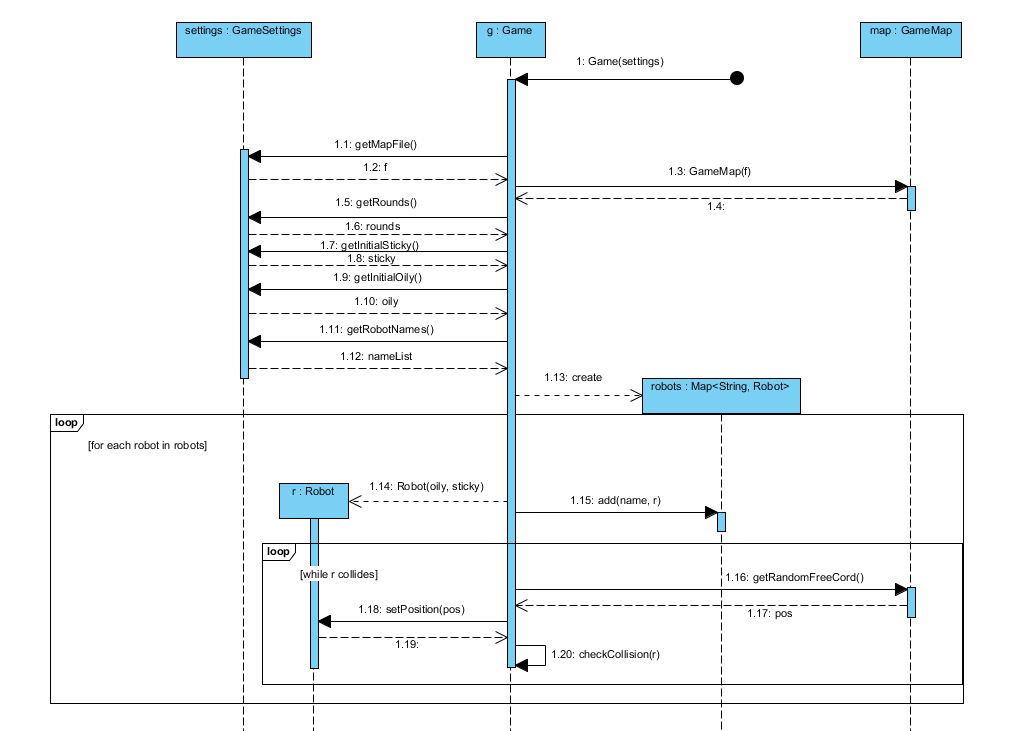
\includegraphics[width=\textwidth, center]{./chapters/chapter03/startgame.png}
	\caption{Játékindítás}
\end{center}
\end{figure}

\begin{figure}[!htbp]
\begin{center}
	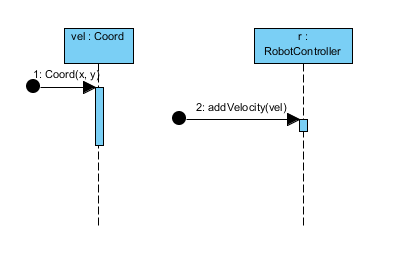
\includegraphics[width=90mm, center]{./chapters/chapter03/velocity.png}
	\caption{Sebességvektor beállítása}
\end{center}
\end{figure}

\clearpage

\begin{figure}[!htbp]
	\begin{center}
		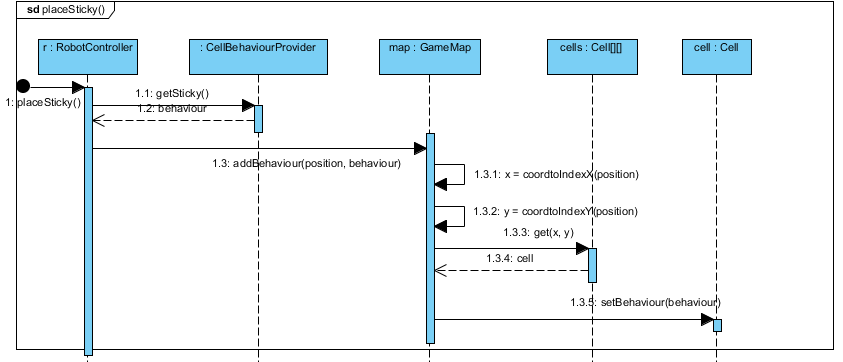
\includegraphics[width=\textwidth, center]{./chapters/chapter03/sticky.png}
		\caption{Ragacs elhelyezése}
	\end{center}
\end{figure}

\begin{figure}[!htbp]
	\begin{center}
		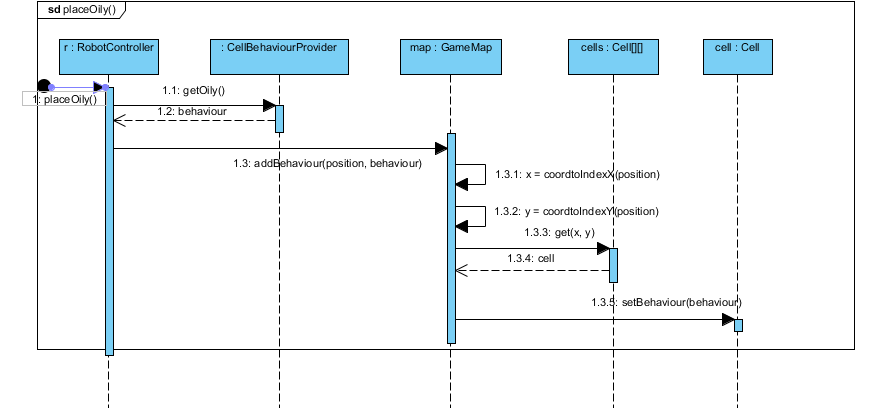
\includegraphics[width=\textwidth, center]{./chapters/chapter03/oily.png}
		\caption{Olaj elhelyezése}
	\end{center}
\end{figure}



\section{State-chartok}
\comment{Csak azokhoz az osztályokhoz, ahol van értelme. Egyetlen állapotból álló state-chartok ne szerepeljenek. A játék működését bemutató state-chart-ot készíteni tilos.}

\begin{figure}[h]
\begin{center}
%\includegraphics[width=17cm]{chapters/chapter03/example.pdf}
\caption{x}
\label{fig:example3}
\end{center}
\end{figure}


% Szglab4
% ===========================================================================
%
\section{Napló}

\begin{naplo}

\bejegyzes
{2015.02.25.~18:00} % Kezdet
{3 óra} % Időtartam
{Pilinszki-Nagy} % Résztvevők
{Tevékenység: A követelmények és szótár javítása a konzultációs utasítások alapján.} % Leírás

\bejegyzes
{2015.02.25.~22:00}
{3 óra}
{Gema}
{Tevékenység: Kezdeti statikus modell felvázolása, kommunikációs platform problémájára megoldás keresése}

\bejegyzes
{2015.02.26.~22:00}
{2 óra}
{Gema, Kemény}
{Tevékenység: Statikus modell korrigálása}

\bejegyzes
{2015.02.27.~15:00} % Kezdet
{5 óra} % Időtartam
{Gema, Kemény} % Résztvevők
{Tevékenység: Statikus modell végleges felépítése.} % Leírás

\bejegyzes
{2015.02.27.~15:30} % Kezdet
{0,5 óra} % Időtartam
{Gema, Juszt, Kemény, Pilinszki-Nagy, Somogyi} % Résztvevők
{Megbeszélés: Feladatok kiosztása a HipChaten keresztül. Döntés: Juszt, Pilinszki-Nagy, Somogyi: 3.1; Gema, Kemény: 3.2; szekvencia diagrammok az elkészült fejezetek alapján.} % Leírás

\bejegyzes
{2015.02.27.~16:00} % Kezdet
{2 óra} % Időtartam
{Juszt, Pilinszki-Nagy, Somogyi} % Résztvevők
{Tevékenység: 3.1, objektum katalógus elkészítése} % Leírás

\bejegyzes
{2015.02.27.~17:30} % Kezdet
{1 óra} % Időtartam
{Somogyi} % Résztvevők
{Tevékenység: Napló vezetése, előző heti feladatok javítása.} % Leírás

\bejegyzes
{2015.02.27.~20:45} % Kezdet
{2 óra} % Időtartam
{Gema, Kemény, Somogyi} % Résztvevők
{Meeting: megbeszélés Google Hangout-on keresztül. Témája: az elkészült statikus modell ismertetése a kollégákkal, a szekvencia diagrammok felépítésének megtervezése.} % Leírás

\bejegyzes
{2015.02.28.~16:00}
{2 óra}
{Gema, Kemény}
{Tevékenység: A dokumentáció 3.2-es pontjának (Osztályok leírása) elkészítése}

\end{naplo}


%
\setcounter{chapter}{3}
	% Szglab4
% ===========================================================================
%
\chapter{Analízis modell kidolgozása 2}

\thispagestyle{fancy}

\section{Objektum katalógus}

\subsection{Robot}

A robotok azok az eszközök, amelyek a játék során versenyeznek egymással. Minden robotra egy felhasználó jut, aki irányíthatja azt. A robotok tudnak elhelyezni a pályán a olajfoltokat és ragacsfoltokat is. A robotok ugrással tudnak a cellákon keresztül a pályán haladni. Minden robotnak van sebessége és természetesen egy aktuális pozíciója is. A robotok tudják magukról, hogy mekkora távolságot tettek már meg a játék során, valamit azt is, hogy még hány olaj- illetve ragacsfolttal rendelkeznek. A robotok egymással ütközhetnek, aminek bekövetkeztekor erről szintén értesülhetnek.

\subsection{Cella}

A cellák tudják magukról, hogy olajfoltosak-e, ragacsfoltosak-e, vagy éppen üresek-e, - azaz egyik folt sem található meg rajtuk. A cellák összessége eredményezi a versenyzésre kijelölt pályát. A cella felelőssége az, hogy ha rálép egy mozgó objektum, akkor annak el tudja végezni a megfelelő utasításait, ilyen például a sebesség megfelezése, folt elhelyezése önmagán, vagy a robotok megsemmisítése.

\subsection{Pálya}

A pálya a cellák összességéből tevődik össze, amiben üres cellák is lesznek, azaz lyukak. Ezen a pályán versenyeznek a robotok valójában. A pálya tisztában van azzal, hogy hol van cella, s hol nincs. (Azaz, hogy melyik koordinátára ugorva marad életben a robot és melyik koordinátára ugorva hal meg.) A pálya tudja megadni az adott koordinátájú cella szomszédos, üresen álló celláit is. Erre akkor van szükség, ha két robot egyszerre szeretne ugyanarra a cellára ugrani. A pálya további felelőssége még, hogy a robotokat egymással összeütköztesse, ha esetleg azonos cellára lépnének. 

\subsection{Olajfolt}

A olajfoltok cellákon helyezkedhetnek el, illetve robotok tudják őket elhelyezni továbblépésük előtt, s ezek módosító hatással vannak az ezt követően belelépő robotokra: a robot sebessége nem lesz módosítható, a következő ugrás sebességvektora így ugyanakkora lesz, mint az előzőé.

\subsection{Ragacsfolt}

A ragacsfoltok szintén a cellákon helyezkedhetnek el, illetve a robotok tudják őket elhelyezni a továbblépésük előtt, s ezek módosító hatással vannak az ezt követően belelépő robotokra: megfelezik a robotok sebességének a nagyságát, tehát lassító hatással bírnak.


\section{Statikus struktúra diagramok}
\comment{Az előző alfejezet osztályainak kapcsolatait és publikus metódusait bemutató osztálydiagram(ok). Tipikus hibalehetőségek: csillag-topológia, szigetek.}

\begin{figure}[h]
\begin{center}
%\includegraphics[width=17cm]{chapters/chapter04/example.pdf}
\caption{x}
\label{fig:example3}
\end{center}
\end{figure}


\section{Osztályok leírása}
\comment{Az előző alfejezetben tárgyalt objektumok felelősségének formalizálása attribútumokká, metódusokká. Csak publikus metódusok szerepelhetnek. Ebben az alfejezetben megjelennek az interfészek, az öröklés, az absztrakt osztályok. Segédosztályokra még mindig nincs szükség. Az osztályok ABC sorrendben kövessék egymást. Interfészek esetén az Interfészek, Attribútumok pontok kimaradnak.}

\subsection{Osztály1}
\begin{itemize}
\item Felelősség\\
\comment{Mi az osztály felelőssége. Kb 1 bekezdés.}
\item Ősosztályok\\
\comment{Mely osztályokból származik (öröklési hierarchia)\newline
Legősebb osztály $\rightarrow$ Ősosztály2 $\rightarrow$ Ősosztály3...}
\item Interfészek\\
\comment{Mely interfészeket valósítja meg.}
\item Attribútumok\\
\comment{Milyen attribútumai vannak}
	\begin{itemize}
		\item attribútum1: attribútum jellemzése: mire való
		\item attribútum2: attribútum jellemzése: mire való
	\end{itemize}
\item Metódusok\\
\comment{Milyen publikus metódusokkal rendelkezik. Metódusonként egy-három mondat arról, hogy a metódus mit csinál.}
	\begin{itemize}
		\item int foo(Osztály3 o1, Osztály4 o2): metódus leírása
		\item int bar(Osztály5 o1): metódus leírása
	\end{itemize}
\end{itemize}

\subsection{Osztály2}
\begin{itemize}
\item Felelősség\\
\comment{Mi az osztály felelőssége. Kb 1 bekezdés.}
\item Ősosztályok\\
\comment{Mely osztályokból származik (öröklési hierarchia)\newline
Legősebb osztály $\rightarrow$ Ősosztály2 $\rightarrow$ Ősosztály3...}
\item Interfészek\\
\comment{Mely interfészeket valósítja meg.}
\item Attribútumok\\
\comment{Milyen attribútumai vannak}
	\begin{itemize}
		\item attribútum1: attribútum jellemzése: mire való
		\item attribútum2: attribútum jellemzése: mire való
	\end{itemize}
\item Metódusok\\
\comment{Milyen publikus metódusokkal rendelkezik. Metódusonként egy-három mondat arról, hogy a metódus mit csinál.}
	\begin{itemize}
		\item int foo(Osztály3 o1, Osztály4 o2): metódus leírása
		\item int bar(Osztály5 o1): metódus leírása
	\end{itemize}
\end{itemize}

\section{Szekvencia diagramok}
\comment{Inicializálásra, use-case-ekre, belső működésre. Konzisztens kell legyen az előző alfejezettel. Minden metódus, ami ott szerepel, fel kell tűnjön valamelyik szekvenciában. Minden metódusnak, ami szekvenciában szerepel, szereplnie kell a valamelyik osztálydiagramon.}

\clearpage

\begin{figure}[!htbp]
	\begin{center}
		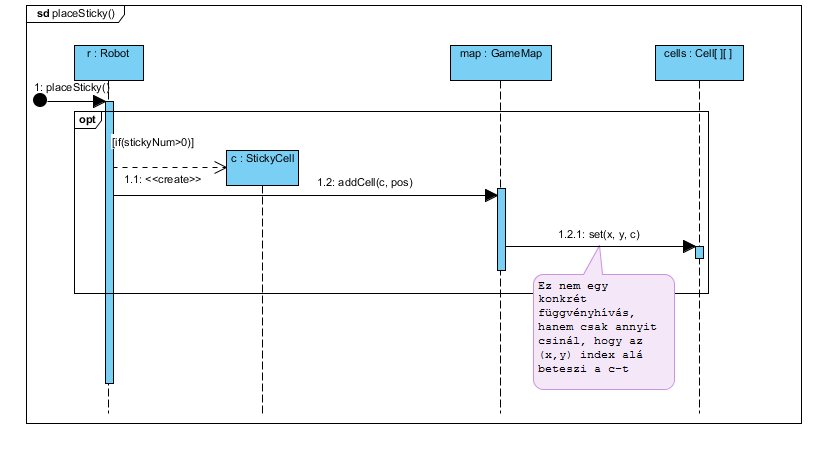
\includegraphics[width=178mm, center]{./chapters/chapter04/sticky.png}
		\caption{Ragacs hátrahagyása}
	\end{center}
\end{figure}

\begin{figure}[!htbp]
	\begin{center}
		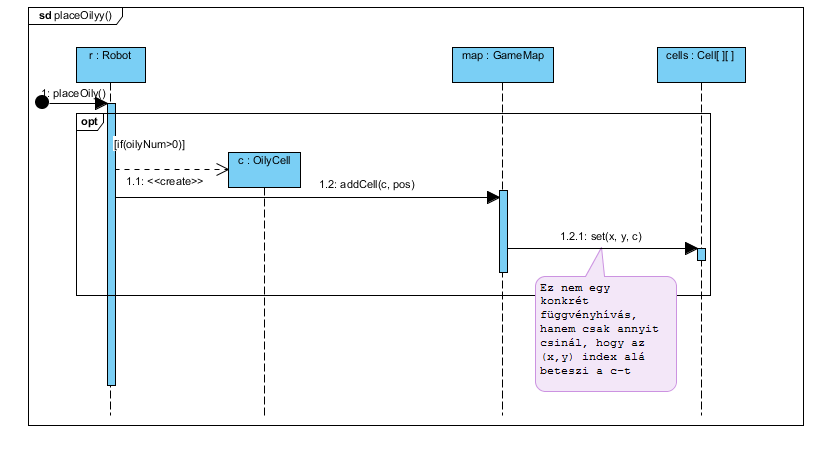
\includegraphics[width=178mm, center]{./chapters/chapter04/oily.png}
		\caption{Olaj hátrahagyása}
	\end{center}
\end{figure}

\begin{figure}[!htbp]
	\begin{center}
		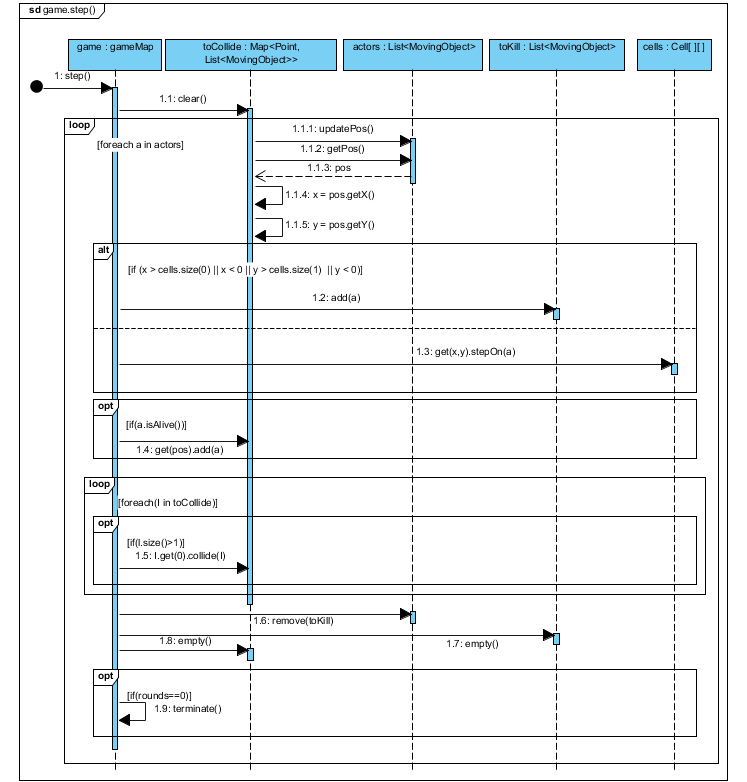
\includegraphics[width=195mm, center]{./chapters/chapter04/step.png}
		\caption{A játék léptetése}
	\end{center}
\end{figure}

\begin{figure}[!htbp]
	\begin{center}
		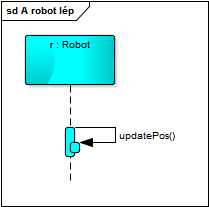
\includegraphics[width=100mm, center]{./chapters/chapter04/Arobotlep.png}
		\caption{}
	\end{center}
\end{figure}

\begin{figure}[!htbp]
	\begin{center}
		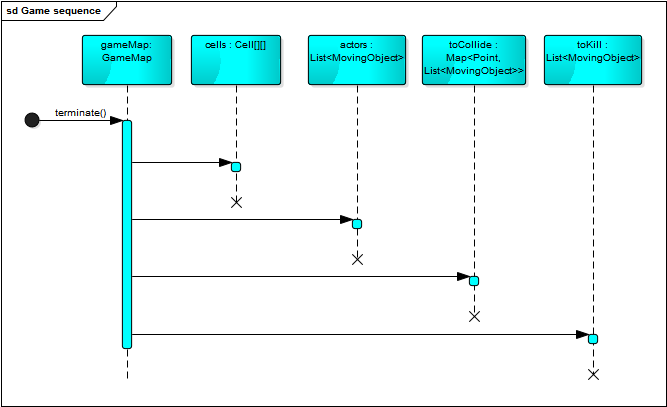
\includegraphics[width=180mm, center]{./chapters/chapter04/Gamesequence.png}
		\caption{}
	\end{center}
\end{figure}

\begin{figure}[!htbp]
	\begin{center}
		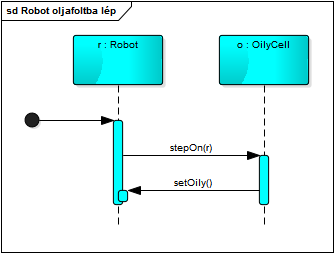
\includegraphics[width=100mm, center]{./chapters/chapter04/robotolajbalep.png}
		\caption{}
	\end{center}
\end{figure}

\begin{figure}[!htbp]
	\begin{center}
		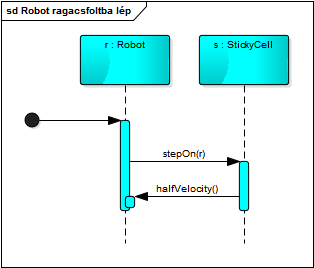
\includegraphics[width=100mm, center]{./chapters/chapter04/robotragacsbalep.png}
		\caption{}
	\end{center}
\end{figure}

\begin{figure}[!htbp]
	\begin{center}
		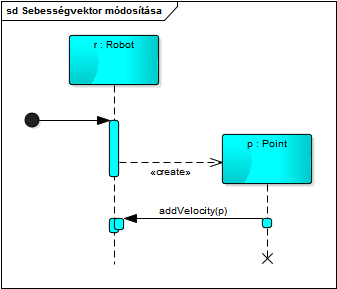
\includegraphics[width=100mm, center]{./chapters/chapter04/sebesseg.png}
		\caption{}
	\end{center}
\end{figure}

\section{State-chartok}
\comment{Csak azokhoz az osztályokhoz, ahol van értelme. Egyetlen állapotból álló state-chartok ne szerepeljenek. A játék működését bemutató state-chart-ot készíteni tilos.}

\begin{figure}[h]
\begin{center}
%\includegraphics[width=17cm]{chapters/chapter04/example.pdf}
\caption{x}
\label{fig:example3}
\end{center}
\end{figure}


% Szglab4
% ===========================================================================
%
\section{Napló}

\begin{naplo}
	
\bejegyzes
{2015.03.04.~12:00~} % Kezdet
{1,5 óra} % Időtartam
{Gema, Juszt, Kemény, Pilinszki-Nagy, Somogyi} % Résztvevők
{Konzultáció: Személyes találkozó a megrendelővel.} % Leírás

\bejegyzes
{2015.03.06.~8:00~} % Kezdet
{2 óra} % Időtartam
{Gema, Juszt, Kemény, Pilinszki-Nagy, Somogyi} % Résztvevők
{Meeting: Stratégiai megbeszélés a munkafolyamatokkal, kommunikációval kapcsolatban, majd a statikus modell felvázolása.} % Leírás

\bejegyzes
{2015.03.06.~20:00~} % Kezdet
{0,5 óra} % Időtartam
{Somogyi} % Résztvevők
{Tevékenység: Objektum katalógus átdolgozása} % Leírás

\bejegyzes
{2015.03.06.~21:00~}
{3 óra}
{Gema, Juszt, Kemény, Pilinszki-Nagy, Somogyi}
{Tevékenység: Statikus modell részletes átdolgozása a kapott instrukciók szerint.}

\bejegyzes
{2015.03.08.~16:00~} % Kezdet
{5 óra} % Időtartam
{Juszt} % Résztvevők
{Új diagramok elkészítése, hibajavítás} % Leírás

\bejegyzes
{2015.03.08.~16:00~} % Kezdet
{5 óra} % Időtartam
{Pilinszki-Nagy} % Résztvevők
{Szekvenciadiagramok készítése, hibák javítása} % Leírás

\bejegyzes
{2015.03.08.~18:00}
{2 óra}
{Somogyi}
{Szekvenciadiagramok készítése, hibák javítása}

\bejegyzes
{2015.03.08.~20:00~} % Kezdet
{4 óra} % Időtartam
{Kemény} % Résztvevők
{Szekvencia diagramok készítése} % Leírás

\bejegyzes
{2015.03.08.~20:00} % kezdet
{5 óra} %Időtartam
{Gema} % Résztvevők
{Osztályok leírásának elkészítése, osztálydiagram véglegesítése és beillesztése a dokumentációba, szekvenciadiagramok ellenőrzése} %Leírás



\end{naplo}


%
\setcounter{chapter}{4}
% Szglab4
% ===========================================================================
%
\chapter{Szkeleton tervezése}

\thispagestyle{fancy}

\section{A szkeleton modell valóságos use-case-ei}

\subsection{Use-case diagram}

\begin{figure}[h]
\begin{center}
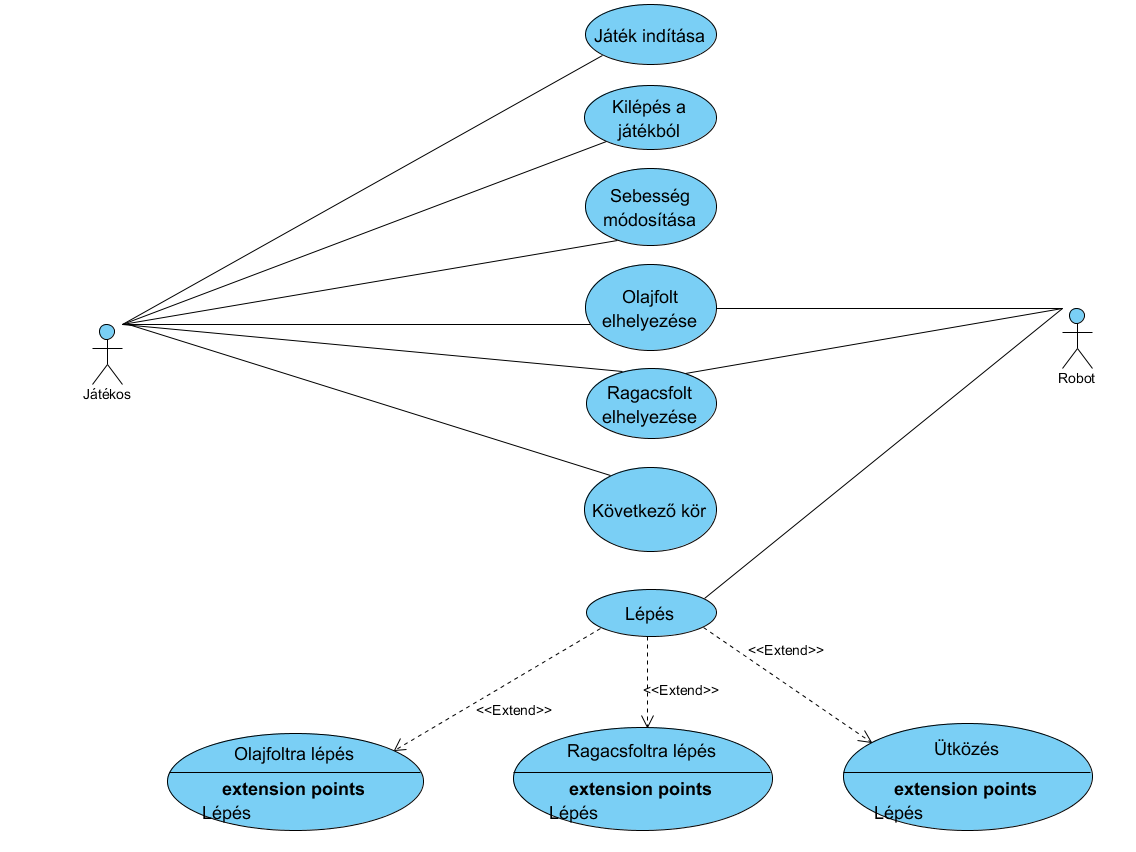
\includegraphics[width=17cm]{chapters/chapter05/use_case.png}
\caption{x}
\label{fig:SzkeletonUseCase}
\end{center}
\end{figure}

\subsection{Use-case leírások}



\usecase{Játék indítása}{Az egyik játékos elindítja a versenyt.}{Felhasználó}{A program menüjéből a felhasználó kiválasztja a Start game funkciót.}

\usecase{Kilépés a játékból}{A felhasználók ki tudnak lépni a játékból.}{Felhasználó}{Ha a játék közben egy játékos úgy dönt, hogy ki szeretne lépni, akkor ezt tudja jelezni és megsemmisül a hozzá tartozó robot.}

\usecase{Sebesség módosítása}{A robot sebesség vektora módosul.}{Játékos, Robot}{Egy játékos megváltoztatja saját robotjának a sebességét, tetszőleges irányú egységvektorral.}

\usecase{Olajfolt elhelyezése}{A robot egy olajfoltot hagy maga után.}{Játékos, Robot}{A játékos utasítására a robot elhelyez egy olajfoltot azon a cellán, amelyiken épp áll.}

\usecase{Ragacsfolt elhelyezése}{A robot egy ragacsfoltot hagy maga után.}{Játékos, Robot}{A játékos utasítására a robot elhelyez egy ragacsfoltot azon a cellán, amelyiken épp áll.}

\usecase{Következő kör}{Léptetés egy körrel.}{Játékos}{Ha minden játékos kiadta a kívánt utasításokat a robotoknak, akkor a kör befejeződik, s egy új kezdődik.}

\usecase{Kiesés a játékból}{Egy robot megsemmisülése.}{Robot}{Ha két robot ütközik, s nincs megfelelő cella számukra, akkor a két robot meghal és kiesik a játékból. Ha egy robot leugrik a kijelölt pályáról, akkor az szintén kiesik a játékból.}

\usecase{Játék megnyerése}{Egy robot megnyeri a játékot.}{Robot}{Ha egy robot marad már csak a pályán, akkor az a robot nyer. Ha elfogy a körök száma, akkor a legnagyobb távolságot megtett, életben maradt robot nyer.}

\usecase{Lépés}{A robot megteszi a lépését.}{Robot}{A robot tovább halad a pályán a megadott sebességvektorral.}

\usecase{Olajfoltra lépés}{A robot rálép egy olajfoltra.}{Robot}{Egy robot egy olajfoltos cellára kénytelen lépni, ezáltal a következő körben a sebessége nem módosítható.}

\usecase{Ragacsfoltra lépés}{A robot rálép egy ragacsfoltra.}{Robot}{Egy robot egy ragacsfoltos cellára kénytelen lépni, ezáltal a sebessége megfeleződik.}

\usecase{Ütközés}{A robotok ütköznek.}{Robot}{Két robot azonos cellára lép, így összeütköznek. Ha a robot egy olyan cellára lép, amelyen már áll egy robot, akkor az ott álló robot továbblép egy véletlenszerűen meghatározott szomszédos cellára. Ha nincs ilyen üres cella, akkor mindkét robot megsemmisül.}


\section{A szkeleton kezelői felületének terve, dialógusok}
A szkeleton egyes funkcióit egy menüből lehet majd elérni a parancssoron keresztül. A program indítása után megjelenik a főmenü a 8 menüponttal, amik közül a menüpont számának megadásával (és egy enter lenyomásával) választhat a felhasználó. A menü a következőképpen fog kinézni:\\

1. Játékindítás\\
\indent \hspace{1 cm}1.1 Cella hozzáadása\\
\indent \hspace{2 cm} 1.1.1 Cella koordinátái szóközzel elválasztva:\\
\indent \hspace{1 cm} 1.2 Robot hozzáadása\\
\indent \hspace{1 cm} 1.3 Főmenübe lépés\\
\indent 2. Robot sebességének módosítása\\
\indent \hspace{1 cm} 2.1 A sebesség koordinátái szóközzel elválasztva:\\
\indent 3. Olajfolt elhelyezése\\
\indent \hspace{1 cm} 3.1 Van olajfoltja a robotnak? $(I/N)$\\
\indent 4. Ragacsfolt elhelyezése\\
\indent \hspace{1 cm} 4.1 Van ragacsfoltja a robotnak? $(I/N$)\\
\indent 5. Következő kör\\
\indent \hspace{1 cm} 5.1 Ez volt az utolsó kör? $(I/N)$\\
\indent 6. Lépés\\
\indent \hspace{1 cm} 6.1 Üres sima cellára lép a robot\\
\indent \hspace{1 cm} 6.2 Ragacsos cellára lép a robot\\
\indent \hspace{1 cm} 6.3 Olajos cellára lép a robot\\
\indent \hspace{1 cm} 6.4 Pályán kívülre lép a robot\\
\indent 7. Ütközés\\
\indent \hspace{1 cm}	7.1 Van elég szabad hely a szomszéd cellákban? $(I/N)$\\	
\indent 8. Kilépés a játékból\\

Az almenüvel rendelkező menüpontok esetén a menüpont kiválasztása után megjelenik az almenü, aminek a kezelése a menüpontoktól függően változik. Abban az esetben, ha egy eldöntendő kérdést ír ki a program, akkor az $I$ billentyűvel adhat igenlő, az $N$ billentyűvel nemleges választ. Ha az almenü további menüpontokat tartalmaz, a főmenüből már ismert módon választhat közülük a felhasználó. (Csak a pont utáni részt szükséges beütnie.) Néhány esetben a program koordinátákat kér, ekkor egy szóközzel elválasztva kell megadni az $x$, majd az $y$ irányú koordinátát. A program itt egy-egy egész számot vár.\\
\par

A futások kimenete egy külső log fájlba fog kerülni, a felhasználó a konzolon keresztül csak arról fog visszajelzést kapni, hogy a végrehajtás részleteit a program kiírta ebbe a fájlba.\\
\par

A kimeneti fájlban az egyes futások elején megtalálható lesz a folyamat ami a konzolon a futtatás előtt lezajlott, valamint ezután az adott futás eredménye, azaz a meghívott függvények nevei. Ezek formátuma a következő lesz: $\left[ :ClassName\right].functionName(\left[ param \right]^*)$, ahol a $ClassName$ az adott osztály nevét, a $functionName$ a hívott függvény nevét, a $param$ kulcsszavak pedig egy-egy paramétert jelölnek. Felüldefiniált függvények esetén mindig a felüldefiniáló osztály neve íródik ki.



\section{Szekvencia diagramok a belső működésre}


\begin{figure}[!htbp]
	\begin{center}
		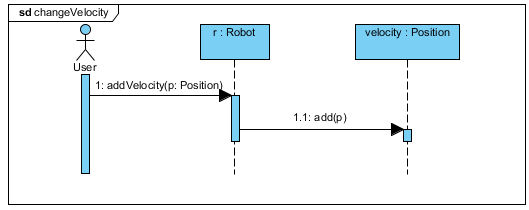
\includegraphics[width=13cm]{./chapters/chapter05/changevelocity.png}
		\caption{Sebesség módosítása}
	\end{center}
\end{figure}

\begin{figure}[!htbp]
	\begin{center}
		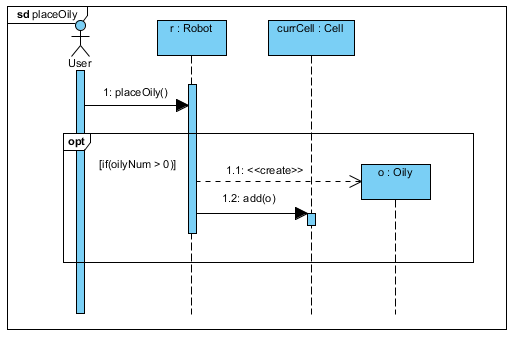
\includegraphics[width=13cm]{./chapters/chapter05/placeoilysequence.png}
		\caption{Olaj lerakása}
	\end{center}
\end{figure}

\begin{figure}[!htbp]
	\begin{center}
		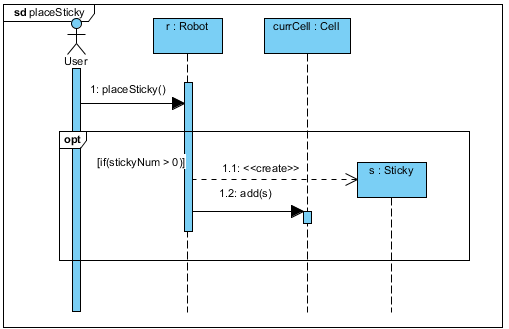
\includegraphics[width=13cm]{./chapters/chapter05/placestickysequence.png}
		\caption{Ragacs lerakása}
	\end{center}
\end{figure}

\clearpage

\begin{figure}[!htbp]
	\begin{center}
		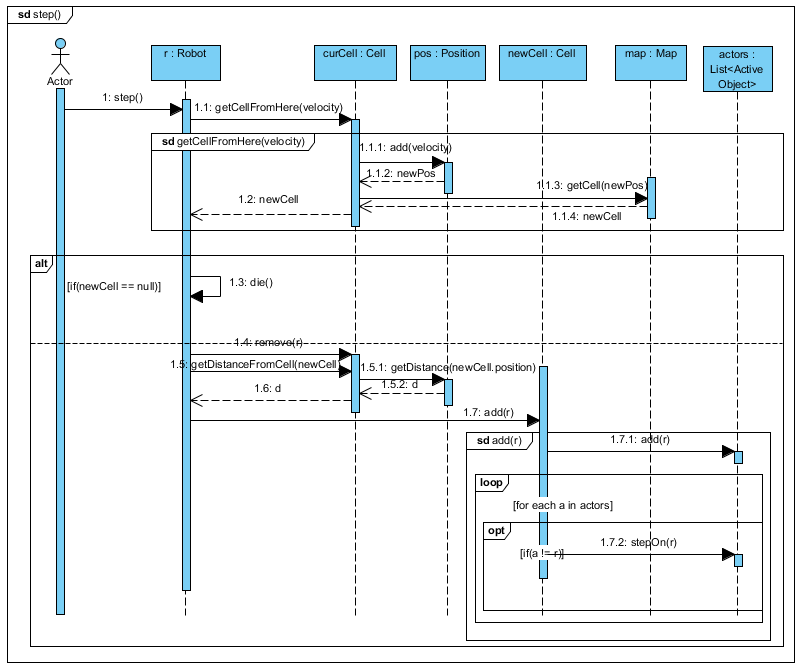
\includegraphics[width=18cm]{./chapters/chapter05/stepsequence.png}
		\caption{Lépés}
	\end{center}
\end{figure}

\clearpage

\begin{figure}[!htbp]
	\begin{center}
		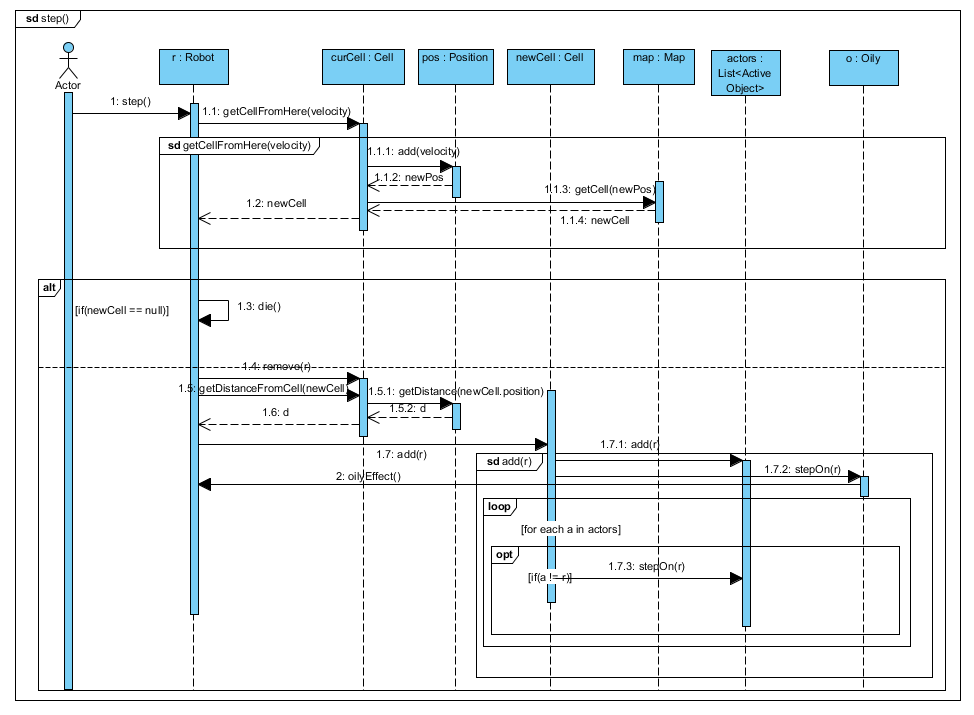
\includegraphics[width=18cm]{./chapters/chapter05/stepoilysequence.png}
		\caption{Lépés olajra}
	\end{center}
\end{figure}

\clearpage

\begin{figure}[!htbp]
	\begin{center}
		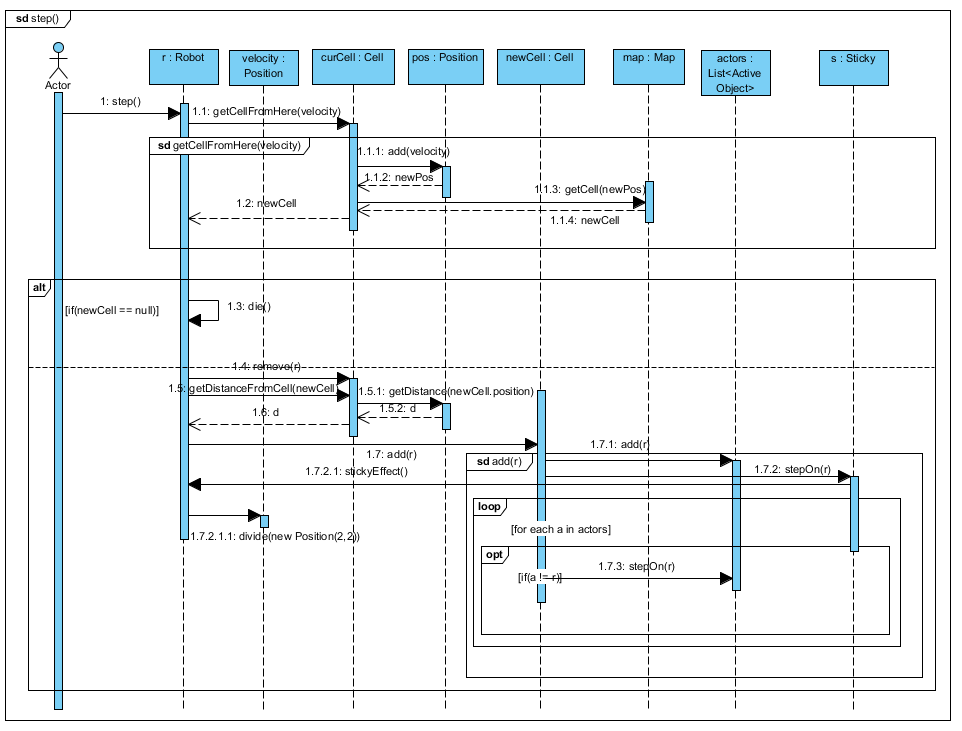
\includegraphics[width=18cm]{./chapters/chapter05/stepstickysequence.png}
		\caption{Lépés ragacsra}
	\end{center}
\end{figure}

\begin{figure}[!htbp]
	\begin{center}
		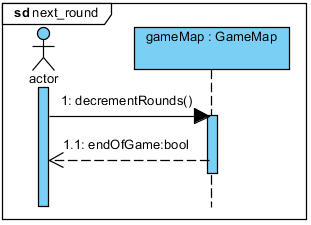
\includegraphics[width=6cm]{./chapters/chapter05/nextround.png}
		\caption{Következő kör}
	\end{center}
\end{figure}


\begin{figure}[!htbp]
	\begin{center}
		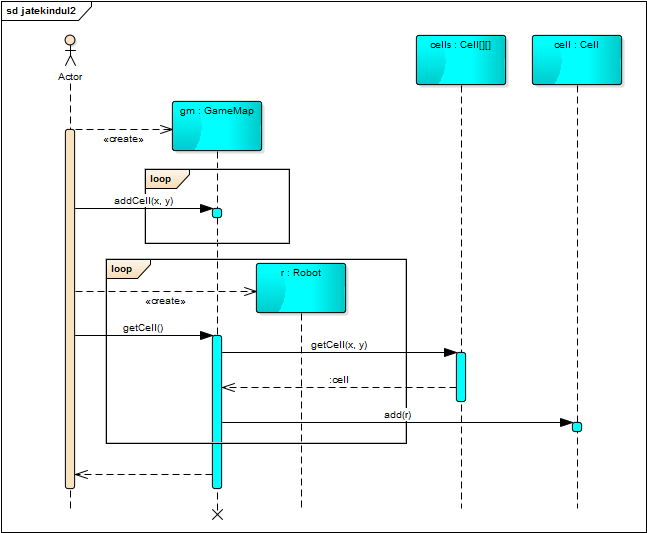
\includegraphics[width=14cm]{./chapters/chapter05/gamestart.png}
		\caption{Játék indítása}
	\end{center}
\end{figure}

\begin{figure}[!htbp]
	\begin{center}
		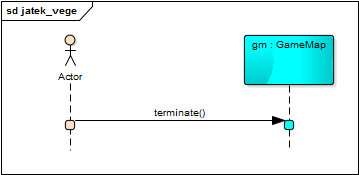
\includegraphics[width=10cm]{./chapters/chapter05/game_end.png}
		\caption{Kilépés a játékból}
	\end{center}
\end{figure}

\clearpage


\begin{figure}[!htbp]
	\begin{center}
		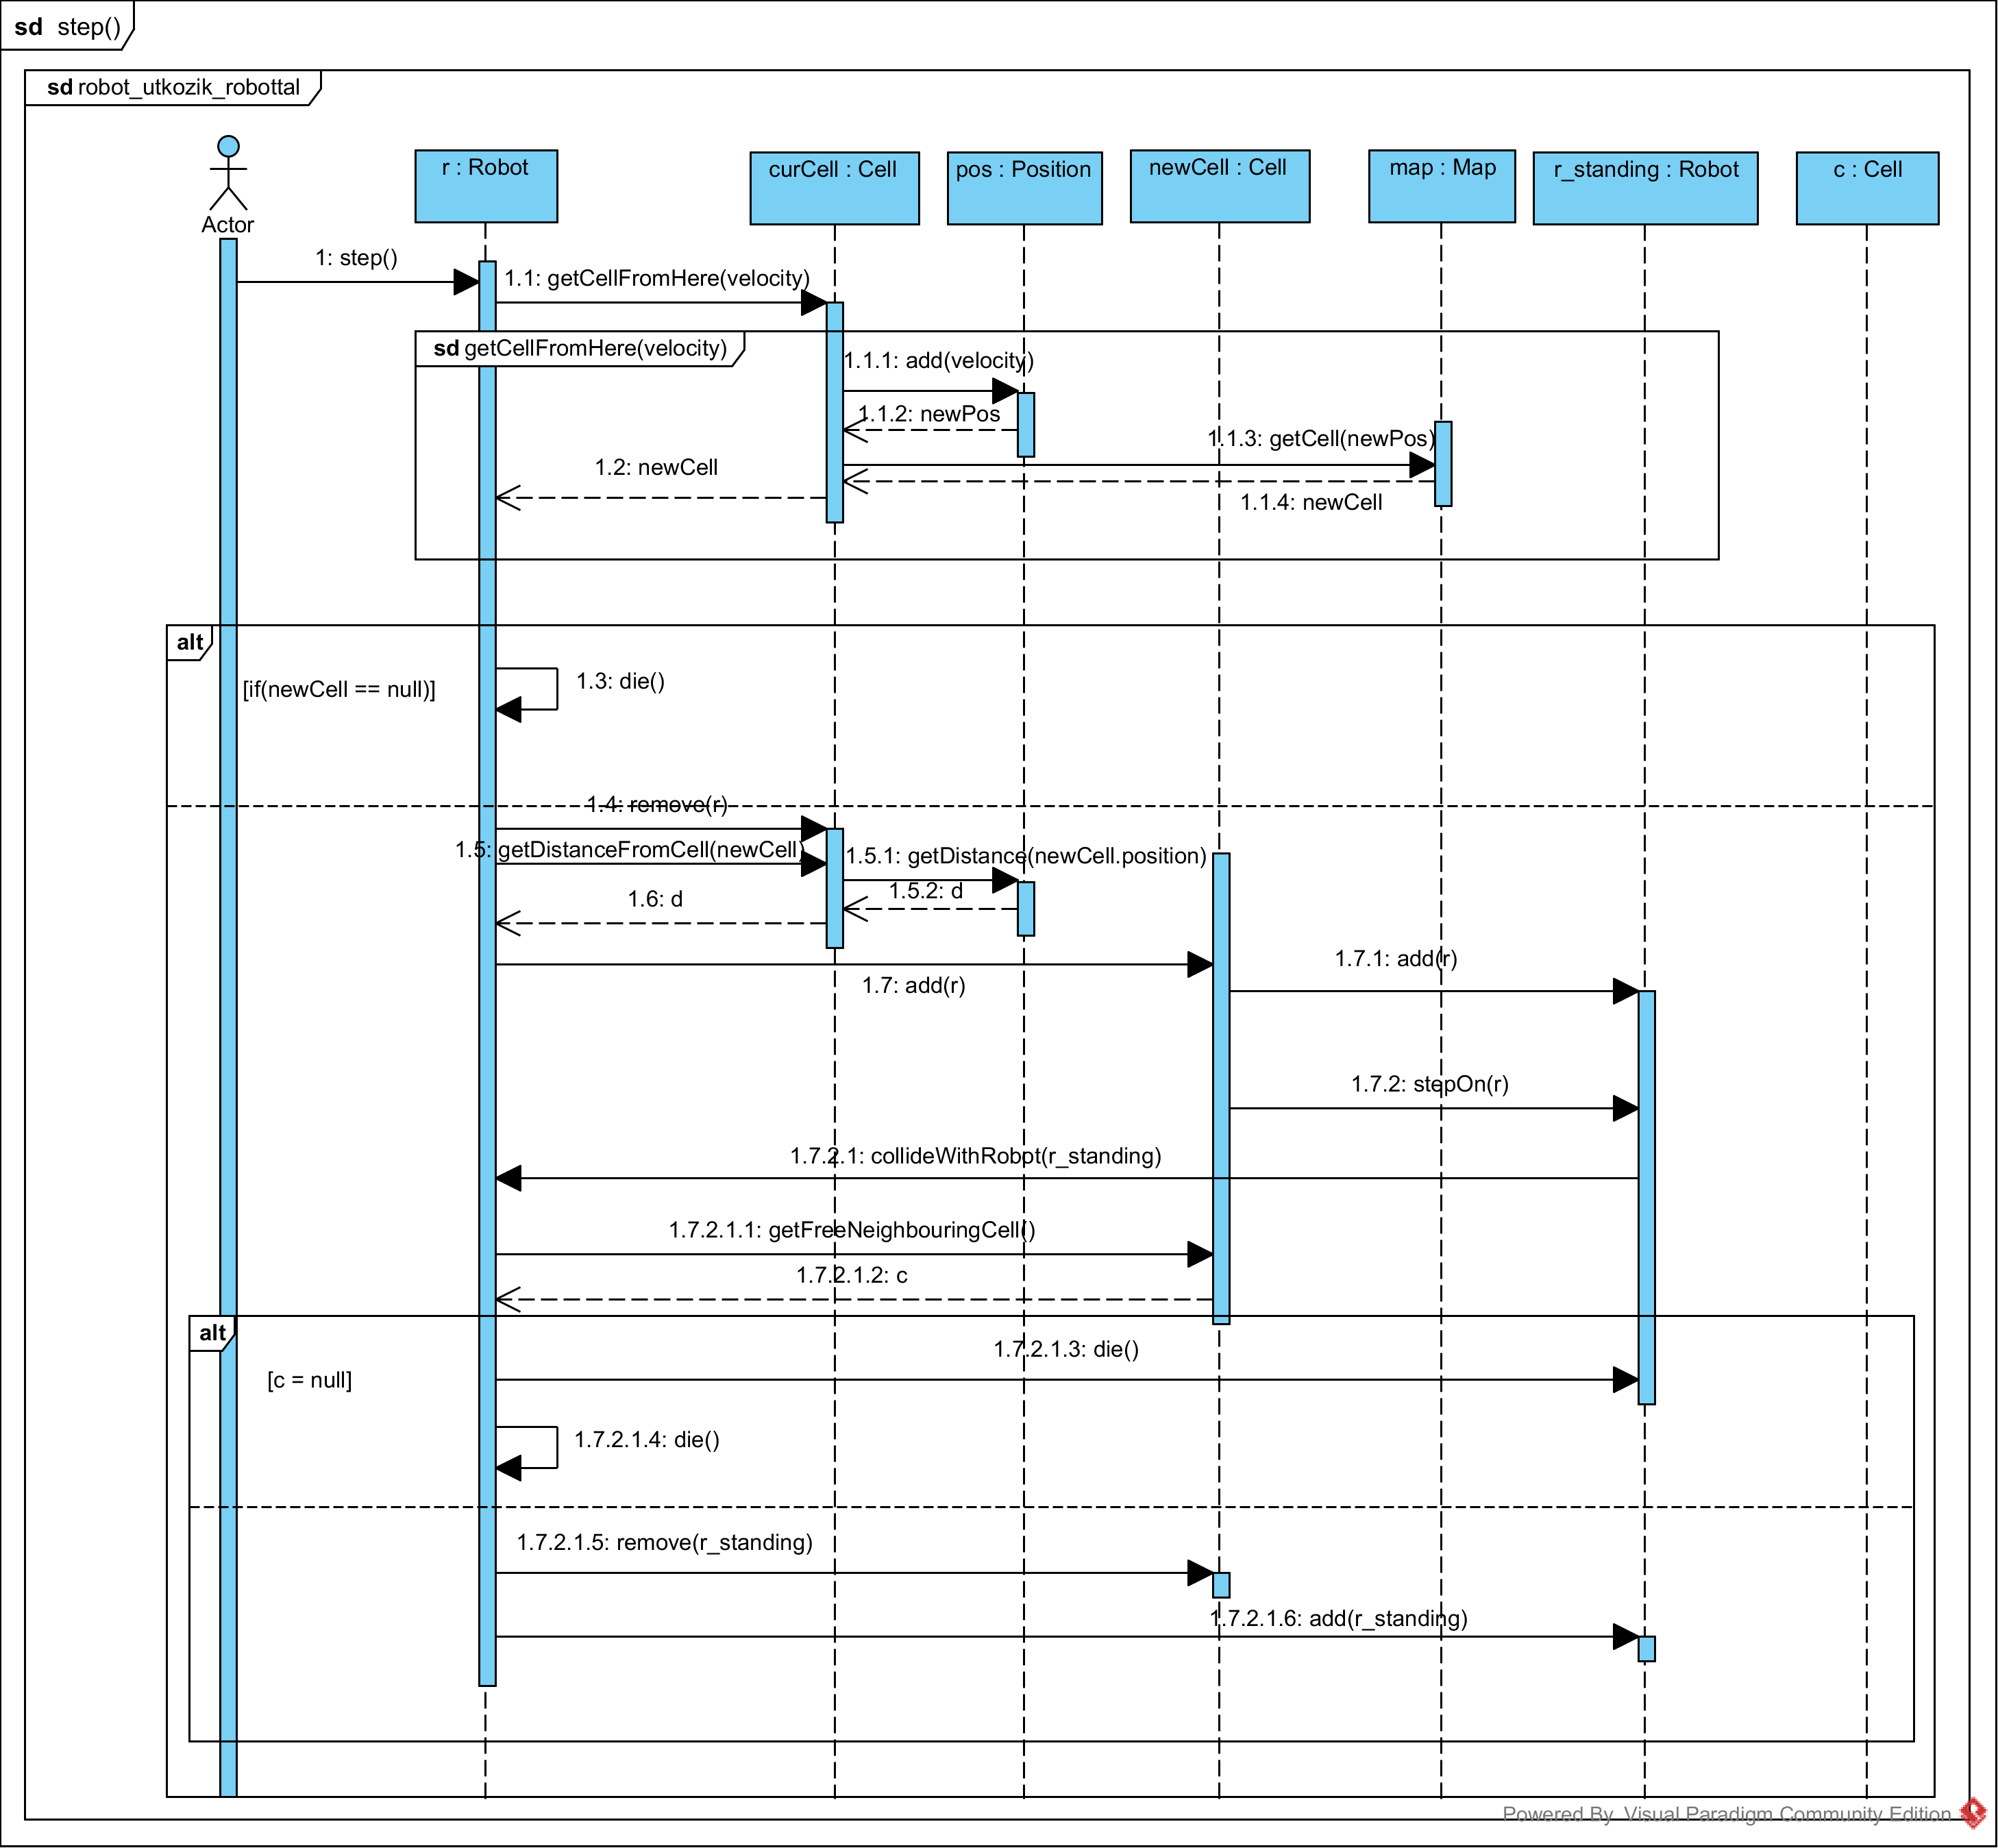
\includegraphics[width=18cm]{./chapters/chapter05/robot_collide_robot.png}
		\caption{Robotok ütköznek}

	\end{center}
\end{figure}

\clearpage

\section{Kommunikációs diagramok}

\begin{figure}[!htbp]
	\begin{center}
		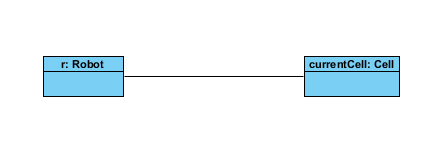
\includegraphics[width=13cm]{./chapters/chapter05/placetrapobject.png}
		\caption{Olajfolt / ragacsfolt lerakása}
	\end{center}
\end{figure}

\begin{figure}[!htbp]
	\begin{center}
		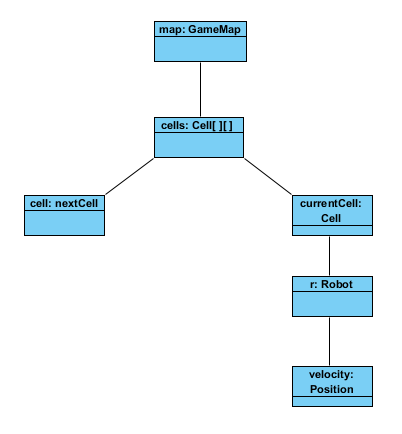
\includegraphics[width=12cm]{./chapters/chapter05/stepobject.png}
		\caption{Lépés, sebesség módosítása}
	\end{center}
\end{figure}


\begin{figure}[!htbp]
	\begin{center}
		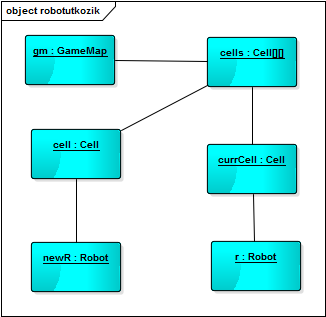
\includegraphics[width=8cm]{./chapters/chapter05/robotutkozikobj.png}
		\caption{Robot ütközik}
	\end{center}
\end{figure}


\begin{figure}[!htbp]
	\begin{center}
		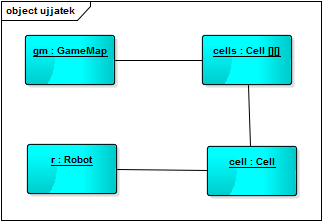
\includegraphics[width=8cm]{./chapters/chapter05/ujjatekobj.png}
		\caption{Új játék}
	\end{center}
\end{figure}

\clearpage

% Szglab4
% ===========================================================================
%
\section{Napló}

\begin{naplo}

\bejegyzes
{2015.03.13.~8:00} % Kezdet
{1,5 óra} % Időtartam
{Juszt, Kemény, Pilinszki-Nagy, Somogyi} % Résztvevők
{Meeting: heti feladatok megbeszélése. Döntés: Juszt, Kemény, Pilinszki-Nagy csinálja a use-case diagramokat, Somogyi a use-case leírásokat.} % Leírás

\bejegyzes
{2015.03.13.~15:00} % Kezdet
{3 óra} % Időtartam
{Kemény} % Résztvevők
{Tevékenység: uj statikus modell elkészítése.} % Leírás

\bejegyzes
{2015.03.13.~19:00} % Kezdet
{2,5 óra} % Időtartam
{Somogyi} % Résztvevők
{Tevékenység: use-case leírások.} % Leírás

\bejegyzes
{2015.03.13.~15:00} % Kezdet
{6 óra} % Időtartam
{Juszt} % Résztvevők
{Tevékenység: múlt heti hibás diagrammok javítása} % Leírás

\bejegyzes
{2015.03.14.~16:00} % Kezdet
{7 óra} % Időtartam
{Juszt} % Résztvevők
{Tevékenység: Új diagrammok elkészítése (szekvencia, objektum)} % Leírás

\bejegyzes
{2015.03.14.~18:00}
{1 óra}
{Gema}
{Tevékenység: Use-case leírások tanulmányozása, módosítási javaslatok összegyűjtése}

\bejegyzes
{2015.03.15.~19:00}
{5 óra}
{Gema}
{Tevékenység: A kiosztott szekvenciadiagramok elkészítése és a szkeleton kezelőfelületének specifikálása}

\bejegyzes
{2015.03.15.~18:00} % Kezdet
{3 óra} % Időtartam
{Kemény} % Résztvevők
{Tevékenység: szekvencia diagramok készítése.} % Leírás

\bejegyzes
{2015.03.15.~12:00} % Kezdet
{10 óra} % Időtartam
{Pilinszki-Nagy} % Résztvevők
{Tevékenység: diagramok készítése(szekvencia, objektum)} % Leírás

\end{naplo}


%
\setcounter{chapter}{5}
% Szglab4
% ===========================================================================
%
\chapter{Szkeleton beadás}

\thispagestyle{fancy}

\section{Fordítási és futtatási útmutató}
\comment{A feltöltött program fordításával és futtatásával kapcsolatos útmutatás. Ennek tartalmaznia kell leltárszerűen az egyes fájlok pontos nevét, méretét byte-ban, keletkezési idejét, valamint azt, hogy a fájlban mi került megvalósításra.}

\subsection{Fájllista}

\begin{fajllista}

\fajl
{Main.java} % Kezdet
{250 byte} % Idptartam
{2009.10.10~18:05~} % Résztvevők
{...} % Leírás

\fajl
{...}
{...}
{...}
{...}

\end{fajllista}

\subsection{Fordítás}
\comment{A fenti listában szereplő forrásfájlokból milyen műveletekkel lehet a bináris, futtatható kódot előállítani. Az előállításhoz csak a 2. Követelmények c. dokumentumban leírt környezetet szabad előírni.}

\lstset{escapeinside=`', xleftmargin=10pt, frame=single, basicstyle=\ttfamily\footnotesize, language=sh}
\begin{lstlisting}
javac -d bin *.java
\end{lstlisting}

\subsection{Futtatás}
\comment{A futtatható kód elindításával kapcsolatos teendők leírása. Az indításhoz csak a 2. Követelmények c. dokumentumban leírt környezetet szabad előírni.}

\lstset{escapeinside=`', xleftmargin=10pt, frame=single, basicstyle=\ttfamily\footnotesize, language=sh}
\begin{lstlisting}
cd bin
java Main.java
\end{lstlisting}

\section{Értékelés}
\comment{A projekt kezdete óta az értékelésig eltelt időben tagokra bontva, százalékban.}

\begin{ertekeles}
\tag{Horváth} % Tag neve
{23.5}        % Munka szazalekban
\tag{Német}
{24.5}
\tag{Tóth}
{25}
\tag{Oláh}
{27}
\end{ertekeles}


% Szglab4
% ===========================================================================
%
\section{Napló}

\begin{naplo}

\bejegyzes
{2010.03.21.~18:00~} % Kezdet
{2,5 óra} % Időtartam
{Horváth\newline
Németh\newline
Tóth\newline
Oláh} % Résztvevők
{Értekezlet. Döntés: Horváth elkészíti az osztálydiagramot, Oláh a use-case leírásokat.} % Leírás

\bejegyzes
{2010.03.23.~23:00~}
{5 óra}
{Németh}
{Tevékenység: Németh implementálja a tesztelő programokat.}

\bejegyzes
{...}
{...}
{...}
{...}


\end{naplo}


%
\setcounter{chapter}{6}
% Szglab4
% ===========================================================================
%
\chapter{Prototípus koncepciója}

\thispagestyle{fancy}

\section{Prototípus interface-definíciója}
\comment{Definiálni kell a teszteket leíró nyelvet. Külön figyelmet kell fordítani arra, hogy ha a rendszer véletlen elemeket is tartalmaz, akkor a véletlenszerűség ki-bekapcsolható legyen, és a program determinisztikusan is tesztelhető legyen.}

\subsection{Az interfész általános leírása}
\comment{A protó (karakteres) input és output felületeit úgy kell kialakítani, hogy az input fájlból is vehető legyen illetőleg az output fájlba menthető legyen, vagyis kommunikációra csak a szabványos be- és kimenet használható.}

\subsection{Bemeneti nyelv}
\comment{Definiálni kell a teszteket leíró nyelvet. Külön figyelmet kell fordítani arra, hogy ha a rendszer véletlen elemeket is tartalmaz, akkor a véletlenszerűség ki-bekapcsolható legyen, és a program determinisztikusan is futtatható legyen. A szálkezelést is tesztelhető, irányítható módon kell megoldani.}

\begin{itemize}
\item Parancs1
	\begin{itemize}
	\item Leírás:
	\item Opciók:
	\end{itemize}
\item Parancs2
	\begin{itemize}
	\item Leírás:
	\item Opciók:
	\end{itemize}

\end{itemize}

\comment{Ha szükséges, meg kell adni a konfigurációs (pl. pályaképet megadó) fájlok nyelvtanát is.}

\subsection{Kimeneti nyelv}
\comment{Egyértelműen definiálni kell, hogy az egyes bemeneti parancsok végrehajtása után előálló állapot milyen formában jelenik meg a szabványos kimeneten.}

\section{Összes részletes use-case}
\comment{A use-case-eknek a részletezettsége feleljen meg a kezelői felületnek, azaz a felület elemeire kell hivatkozniuk.
Alábbi táblázat minden use-case-hez külön-külön.}

\begin{figure}[h]
\begin{center}
%\includegraphics[width=17cm]{chapters/chapter07/example.pdf}
\caption{x}
\label{fig:ProtoUseCase}
\end{center}
\end{figure}

\usecase{...}{...}{...}{...}

\section{Tesztelési terv}
\comment{A tesztelési tervben definiálni kell, hogy a be- és kimeneti fájlok egybevetésével miként végezhető el a program tesztelése. Meg kell adni teszt forgatókönyveket. Az egyes teszteket elég informálisan, szabad szövegként leírni. Teszt-esetenként egy-öt mondatban. Minden teszthez meg kell adni, hogy mi a célja, a proto mely funkcionalitását, osztályait stb. teszteli. Az alábbi táblázat minden teszt-esethez külön-külön elkészítendő.}

\teszteset{...}{...}{...}

\section{Tesztelést támogató segéd- és fordítóprogramok specifikálása}
\comment{Specifikálni kell a tesztelést támogató segédprogramokat.}


% Szglab4
% ===========================================================================
%
\section{Napló}

\begin{naplo}

\bejegyzes
{2010.03.21.~18:00~} % Kezdet
{2,5 óra} % Időtartam
{Horváth\newline
Németh\newline
Tóth\newline
Oláh} % Résztvevők
{Értekezlet. Döntés: Horváth elkészíti az osztálydiagramot, Oláh a use-case leírásokat.} % Leírás

\bejegyzes
{2010.03.23.~23:00~}
{5 óra}
{Németh}
{Tevékenység: Németh implementálja a tesztelő programokat.}

\bejegyzes
{...}
{...}
{...}
{...}


\end{naplo}


%
\setcounter{chapter}{7}
% Szglab4
% ===========================================================================
%
\chapter{Részletes tervek}

\thispagestyle{fancy}

\section{Osztályok és metódusok tervei}

\subsection{Osztály1}
\begin{itemize}
\item Felelősség\newline
\comment{Mi az osztály felelőssége. Kb 1 bekezdés. Ha szükséges, akkor state-chart is.}
\item Ősosztályok\newline
\comment{Mely osztályokból származik (öröklési hierarchia)\newline
Legősebb osztály $\rightarrow$ Ősosztály2 $\rightarrow$ Ősosztály3...}
\item Interfészek\newline
\comment{Mely interfészeket valósítja meg.}
\item Attribútumok\newline
\comment{Milyen attribútumai vannak}
	\begin{itemize}
		\item attribútum1: attribútum jellemzése: mire való, láthatósága (UML jelöléssel), típusa
		\item attribútum2: attribútum jellemzése: mire való, láthatósága (UML jelöléssel), típusa
	\end{itemize}
\item Metódusok\newline
\comment{Milyen publikus, protected és privát  metódusokkal rendelkezik. Metódusonként precíz leírás, ha szükséges, activity diagram is  a metódusban megvalósítandó algoritmusról.}
	\begin{itemize}
		\item int foo(Osztály3 o1, Osztály4 o2): metódus leírása, láthatósága (UML jelöléssel)
		\item int bar(Osztály5 o1): metódus leírása, láthatósága (UML jelöléssel)
	\end{itemize}
\end{itemize}

\subsection{Osztály2}
\begin{itemize}
\item Felelősség\newline
\comment{Mi az osztály felelőssége. Kb 1 bekezdés. Ha szükséges, akkor state-chart is.}
\item Ősosztályok\newline
\comment{Mely osztályokból származik (öröklési hierarchia)\newline
Legősebb osztály $\rightarrow$ Ősosztály2 $\rightarrow$ Ősosztály3...}
\item Interfészek\newline
\comment{Mely interfészeket valósítja meg.}
\item Attribútumok\newline
\comment{Milyen attribútumai vannak}
	\begin{itemize}
		\item attribútum1: attribútum jellemzése: mire való, láthatósága (UML jelöléssel), típusa
		\item attribútum2: attribútum jellemzése: mire való, láthatósága (UML jelöléssel), típusa
	\end{itemize}
\item Metódusok\newline
\comment{Milyen publikus, protected és privát  metódusokkal rendelkezik. Metódusonként precíz leírás, ha szükséges, activity diagram is  a metódusban megvalósítandó algoritmusról.}
	\begin{itemize}
		\item int foo(Osztály3 o1, Osztály4 o2): metódus leírása, láthatósága (UML jelöléssel)
		\item int bar(Osztály5 o1): metódus leírása, láthatósága (UML jelöléssel)
	\end{itemize}
\end{itemize}

\section{A tesztek részletes tervei, leírásuk a teszt nyelvén}
[A tesztek részletes tervei alatt meg kell adni azokat a bemeneti adatsorozatokat, amelyekkel a program működése ellenőrizhető. Minden bemenő adatsorozathoz definiálni kell, hogy az adatsorozat végrehajtásától a program mely részeinek, funkcióinak ellenőrzését várjuk és konkrétan milyen eredményekre számítunk, ezek az eredmények hogyan vethetők össze a bemenetekkel.]

\subsection{Teszteset1}
\begin{itemize}
\item Leírás\newline
\comment{szöveges leírás, kb. 1-5 mondat.}
\item Ellenőrzött funkcionalitás, várható hibahelyek
\item Bemenet\newline
\comment{a proto bemeneti nyelvén megadva (lásd előző anyag)}
\item Elvárt kimenet\newline
\comment{a proto kimeneti nyelvén megadva (lásd előző anyag)}
\end{itemize}

\subsection{Teszteset2}
\begin{itemize}
\item Leírás\newline
\comment{szöveges leírás, kb. 1-5 mondat.}
\item Ellenőrzött funkcionalitás, várható hibahelyek
\item Bemenet\newline
\comment{a proto bemeneti nyelvén megadva (lásd előző anyag)}
\item Elvárt kimenet\newline
\comment{a proto kimeneti nyelvén megadva (lásd előző anyag)}
\end{itemize}

\section{A tesztelést támogató programok tervei}
\comment{A tesztadatok előállítására, a tesztek eredményeinek kiértékelésére szolgáló segédprogramok részletes terveit kell elkészíteni.}


% Szglab4
% ===========================================================================
%
\section{Napló}

\begin{naplo}

\bejegyzes
{2010.03.21.~18:00~} % Kezdet
{2,5 óra} % Időtartam
{Horváth\newline
Németh\newline
Tóth\newline
Oláh} % Résztvevők
{Értekezlet. Döntés: Horváth elkészíti az osztálydiagramot, Oláh a use-case leírásokat.} % Leírás

\bejegyzes
{2010.03.23.~23:00~}
{5 óra}
{Németh}
{Tevékenység: Németh implementálja a tesztelő programokat.}

\bejegyzes
{...}
{...}
{...}
{...}


\end{naplo}


%
\setcounter{chapter}{9}
% Szglab4
% ===========================================================================
%
\chapter{Prototípus beadása}

\thispagestyle{fancy}

\section{Fordítási és futtatási útmutató}
\comment{A feltöltött program fordításával és futtatásával kapcsolatos útmutatás. Ennek tartalmaznia kell leltárszerűen az egyes fájlok pontos nevét, méretét byte-ban, keletkezési idejét, valamint azt, hogy a fájlban mi került megvalósításra.}

\subsection{Fájllista}

\begin{fajllista}

\fajl
{Main.java} % Kezdet
{250 byte} % Idptartam
{2009.10.10~18:05~} % Résztvevők
{...} % Leírás

\fajl
{...}
{...}
{...}
{...}

\end{fajllista}

\subsection{Fordítás}
\comment{A fenti listában szereplő forrásfájlokból milyen műveletekkel lehet a bináris, futtatható kódot előállítani. Az előállításhoz csak a 2. Követelmények c. dokumentumban leírt környezetet szabad előírni.}

\lstset{escapeinside=`', xleftmargin=10pt, frame=single, basicstyle=\ttfamily\footnotesize, language=sh}
\begin{lstlisting}
javac -d bin *.java
\end{lstlisting}

\subsection{Futtatás}
\comment{A futtatható kód elindításával kapcsolatos teendők leírása. Az indításhoz csak a 2. Követelmények c. dokumentumban leírt környezetet szabad előírni.}

\lstset{escapeinside=`', xleftmargin=10pt, frame=single, basicstyle=\ttfamily\footnotesize, language=sh}
\begin{lstlisting}
cd bin
java Main.java
\end{lstlisting}


\section{Tesztek jegyzőkönyvei}

\subsection{Teszteset1}
\comment{Az alábbi táblázatot az utolsó, sikeres tesztfuttatáshoz kell kitölteni}

\tesztok{...}{...}

\comment{Az alábbi táblázatot a megismételt (hibás) tesztek esetén kell kitölteni minden ismétléshez egyszer. Ha szükséges, akkor a valós kimenet is mellékelhető mint a teszt eredménye.}

\tesztfail{...}{...}{...}{...}{...}

\section{Értékelés}
\comment{A projekt kezdete óta az értékelésig eltelt időben tagokra bontva, százalékban.}

\begin{ertekeles}
\tag{Horváth} % Tag neve
{23.5}        % Munka szazalekban
\tag{Német}
{24.5}
\tag{Tóth}
{25}
\tag{Oláh}
{27}
\end{ertekeles}


% Szglab4
% ===========================================================================
%
\section{Napló}

\begin{naplo}

\bejegyzes
{2010.03.21.~18:00~} % Kezdet
{2,5 óra} % Időtartam
{Horváth\newline
Németh\newline
Tóth\newline
Oláh} % Résztvevők
{Értekezlet. Döntés: Horváth elkészíti az osztálydiagramot, Oláh a use-case leírásokat.} % Leírás

\bejegyzes
{2010.03.23.~23:00~}
{5 óra}
{Németh}
{Tevékenység: Németh implementálja a tesztelő programokat.}

\bejegyzes
{...}
{...}
{...}
{...}


\end{naplo}


%
\setcounter{chapter}{10}
% Szglab4
% ===========================================================================
%
\chapter{Grafikus felület specifikációja}

\thispagestyle{fancy}

\section{A grafikus interfész}
\comment{A menürendszer, a kezelői felület grafikus képe. A grafikus felület megjelenését, a használt ikonokat, stb screenshot-szerű képekkel kell bemutatni. Az építészetben ez a homlokzati terv.}

\begin{figure}[h]
\begin{center}
%\includegraphics[width=17cm]{chapters/chapter11/example.pdf}
\caption{x}
\label{fig:Grafikus}
\end{center}
\end{figure}

\section{A grafikus rendszer architektúrája}
\comment{A felület működésének elve, a grafikus rendszer architektúrája (struktúra diagramok). A struktúra diagramokon a prototípus azon és csak azon osztályainak is szerepelnie kell, amelyekhez a grafikus felületet létrehozó osztályok kapcsolódnak.}

\subsection{A felület működési elve}
\comment{Le kell írni, hogy a grafikai megjelenésért felelős osztályok, objektumok hogyan kapcsolódnak a meglevő rendszerhez, a megjelenítés során mi volt az alapelv. Törekedni kell az MVC megvalósításra. Alapelvek lehetnek: \textbf{push} alapú: a modell értesíti a felületet, hogy változott; \textbf{pull} alapú: a felület kérdezi le a modellt, hogy változott-e; \textbf{kevert}: a kettő kombinációja.}

\subsection{A felület osztály-struktúrája}
\comment{Osztálydiagram. Minden új osztály, és azon régiek, akik az újakhoz közvetlenül kapcsolódnak.}

\section{A grafikus objektumok felsorolása}
\comment{Az új osztályok felsorolása. Az régi osztályok közül azoknak a felsorolása, ahol változás volt. Ezek esetén csak a változásokat kell leírni.}

\subsection{Osztály1}
\begin{itemize}
\item Felelősség\newline
\comment{Mi az osztály felelőssége. Kb 1 bekezdés. Ha szükséges, akkor state-chart is.}
\item Ősosztályok\newline
\comment{Mely osztályokból származik (öröklési hierarchia)\newline
Legősebb osztály $\rightarrow$ Ősosztály2 $\rightarrow$ Ősosztály3...}
\item Interfészek\newline
\comment{Mely interfészeket valósítja meg.}
\item Attribútumok\newline
\comment{Milyen attribútumai vannak}
	\begin{itemize}
		\item attribútum1: attribútum jellemzése: mire való, láthatósága (UML jelöléssel), típusa
		\item attribútum2: attribútum jellemzése: mire való, láthatósága (UML jelöléssel), típusa
	\end{itemize}
\item Metódusok\newline
\comment{Milyen publikus, protected és privát  metódusokkal rendelkezik. Metódusonként precíz leírás, ha szükséges, activity diagram is  a metódusban megvalósítandó algoritmusról.}
	\begin{itemize}
		\item int foo(Osztály3 o1, Osztály4 o2): metódus leírása, láthatósága (UML jelöléssel)
		\item int bar(Osztály5 o1): metódus leírása, láthatósága (UML jelöléssel)
	\end{itemize}
\end{itemize}

\subsection{Osztály2}
\begin{itemize}
\item Felelősség\newline
\comment{Mi az osztály felelőssége. Kb 1 bekezdés. Ha szükséges, akkor state-chart is.}
\item Ősosztályok\newline
\comment{Mely osztályokból származik (öröklési hierarchia)\newline
Legősebb osztály $\rightarrow$ Ősosztály2 $\rightarrow$ Ősosztály3...}
\item Interfészek\newline
\comment{Mely interfészeket valósítja meg.}
\item Attribútumok\newline
\comment{Milyen attribútumai vannak}
	\begin{itemize}
		\item attribútum1: attribútum jellemzése: mire való, láthatósága (UML jelöléssel), típusa
		\item attribútum2: attribútum jellemzése: mire való, láthatósága (UML jelöléssel), típusa
	\end{itemize}
\item Metódusok\newline
\comment{Milyen publikus, protected és privát  metódusokkal rendelkezik. Metódusonként precíz leírás, ha szükséges, activity diagram is  a metódusban megvalósítandó algoritmusról.}
	\begin{itemize}
		\item int foo(Osztály3 o1, Osztály4 o2): metódus leírása, láthatósága (UML jelöléssel)
		\item int bar(Osztály5 o1): metódus leírása, láthatósága (UML jelöléssel)
	\end{itemize}
\end{itemize}

\section{Kapcsolat az alkalmazói rendszerrel}
\comment{Szekvencia-diagramokon ábrázolni kell a grafikus rendszer működését. Konzisztens kell legyen az előző alfejezetekkel. Minden metódus, ami ott szerepel, fel kell tűnjön valamelyik szekvenciában. Minden metódusnak, ami szekvenciában szerepel, szereplnie kell a valamelyik osztálydiagramon.}


% Szglab4
% ===========================================================================
%
\section{Napló}

\begin{naplo}

\bejegyzes
{2010.03.21.~18:00~} % Kezdet
{2,5 óra} % Időtartam
{Horváth\newline
Németh\newline
Tóth\newline
Oláh} % Résztvevők
{Értekezlet. Döntés: Horváth elkészíti az osztálydiagramot, Oláh a use-case leírásokat.} % Leírás

\bejegyzes
{2010.03.23.~23:00~}
{5 óra}
{Németh}
{Tevékenység: Németh implementálja a tesztelő programokat.}

\bejegyzes
{...}
{...}
{...}
{...}


\end{naplo}


%
\setcounter{chapter}{12}
% Szglab4
% ===========================================================================
%
\chapter{Grafikus felület specifikációja}

\thispagestyle{fancy}

\section{Fordítási és futtatási útmutató}
\comment{A feltöltött program fordításával és futtatásával kapcsolatos útmutatás. Ennek tartalmaznia kell leltárszerűen az egyes fájlok pontos nevét, méretét byte-ban, keletkezési idejét, valamint azt, hogy a fájlban mi került megvalósításra.}

\subsection{Fájllista}

\begin{fajllista}

\fajl
{Main.java} % Kezdet
{250 byte} % Idptartam
{2009.10.10~18:05~} % Résztvevők
{...} % Leírás

\fajl
{...}
{...}
{...}
{...}

\end{fajllista}

\subsection{Fordítás}
\comment{A fenti listában szereplő forrásfájlokból milyen műveletekkel lehet a bináris, futtatható kódot előállítani. Az előállításhoz csak a 2. Követelmények c. dokumentumban leírt környezetet szabad előírni.}

\lstset{escapeinside=`', xleftmargin=10pt, frame=single, basicstyle=\ttfamily\footnotesize, language=sh}
\begin{lstlisting}
javac -d bin *.java
\end{lstlisting}

\subsection{Futtatás}
\comment{A futtatható kód elindításával kapcsolatos teendők leírása. Az indításhoz csak a 2. Követelmények c. dokumentumban leírt környezetet szabad előírni.}

\lstset{escapeinside=`', xleftmargin=10pt, frame=single, basicstyle=\ttfamily\footnotesize, language=sh}
\begin{lstlisting}
cd bin
java Main.java
\end{lstlisting}

\section{Értékelés}
\comment{A projekt kezdete óta az értékelésig eltelt időben tagokra bontva, százalékban.}

\begin{ertekeles}
\tag{Horváth} % Tag neve
{23.5}        % Munka szazalekban
\tag{Német}
{24.5}
\tag{Tóth}
{25}
\tag{Oláh}
{27}
\end{ertekeles}


% Szglab4
% ===========================================================================
%
\section{Napló}

\begin{naplo}

\bejegyzes
{2010.03.21.~18:00~} % Kezdet
{2,5 óra} % Időtartam
{Horváth\newline
Németh\newline
Tóth\newline
Oláh} % Résztvevők
{Értekezlet. Döntés: Horváth elkészíti az osztálydiagramot, Oláh a use-case leírásokat.} % Leírás

\bejegyzes
{2010.03.23.~23:00~}
{5 óra}
{Németh}
{Tevékenység: Németh implementálja a tesztelő programokat.}

\bejegyzes
{...}
{...}
{...}
{...}


\end{naplo}


%
\setcounter{chapter}{13}
% Szglab4
% ===========================================================================
%
\chapter{Összefoglalás}

\thispagestyle{fancy}

\section{Projekt összegzés}
\comment{A projekt tapasztalatait összegző részben a csapatoknak a projektről kialakult véleményét várjuk. A megválaszolandók köre az alábbi. }

\begin{munka}
\munkaido{Horváth}{98}
\munkaido{Németh}{95}
\munkaido{Tóth}{102}
\munkaido{Oláh}{87}
\osszesmunkaido{382}
\end{munka}

\begin{forrassor}
\munkaido{Szkeleton}{500}
\munkaido{Protó}{600}
\munkaido{Grafikus}{700}
\end{forrassor}

\begin{itemize}
\item Mit tanultak a projektből konkrétan és általában? \newline
\item Mi volt a legnehezebb és a legkönnyebb? \newline
\item Összhangban állt-e az idő és a pontszám az elvégzendő feladatokkal? \newline
\item Ha nem, akkor hol okozott ez nehézséget? \newline
\item Milyen változtatási javaslatuk van? \newline
\item Milyen feladatot ajánlanának a projektre? \newline
\end{itemize}

\comment{Szívesen fogadunk minden egyéb kritikát és javaslatot.}


%

%\clearpage
%
% Függelék
%
%\appendix

\end{document}
%
% EOF
%
